    \documentclass[12pt]{article}
    
    %AMS-TeX packages
    \usepackage{amssymb,amsmath,amsthm} 
    \usepackage{geometry, graphicx}
    \usepackage{tabulary}
    \usepackage{upgreek}
    \usepackage{siunitx}
    \usepackage{caption}
    \usepackage{subcaption}
    \usepackage{csvsimple}
    \usepackage{enumitem}
    
    \sisetup{locale=US,group-separator = {,}, math-micro={\upmu}}
    
    \usepackage{pgfplotstable,filecontents}
    \pgfplotsset{compat=1.9}% supress warning
    
    % setup the margins
\geometry{margin=1.0in, headheight=15pt}
    
    
\graphicspath{ {../lab02/images} }    
    
    \begin{document}
    
    \title{PHSX 444: Lab 02; Fourier Transforms}
    \author{William Jardee}
    \maketitle
    
    %% Introduction section. Here I introduce the physics of the experiment and give some slight motivation for the experiment. I personally think that putting the physics of the apparatus here is better. 
    \section{Introduction}
    
    One of the neatest characteristics of orthogonal basises is how they can be used to recreate a wide range of functions. Probably the most notable of all these basises is the fourier transform. As can be shown through a relatively simple, but clever, derivation, all functions can be written as:
    \begin{equation*}
        Y(t) = \int^\infty_{-\infty} y(t) \frac{e^{-i\omega t}}{\sqrt{2\pi}} dt
        \label{eq:fourier_time}
    \end{equation*}
    \begin{equation*}
        y(t) = \int^\infty_{-\infty} Y(\omega) \frac{e^{-i\omega t}}{\sqrt{2\pi}} dt
        \label{eq:fourier_freq}
    \end{equation*}
    This isn't all too useful in application, however. There are two issues here. The first requiring an exact knowledge of the function to begin with, either in the frequency or time domain. The second being the computation time of finding such a solution to the equation (or the discrete version that we will see).
    
    To solve the first issue, the Fourier Transform can be rewritten as the Discrete Fourier Transform:
    \begin{equation*}
        Y(t) = \sum^{N-1}_{k=0} \Delta t \cdot \frac{e^{i \omega_n t_k}}{\sqrt{2\pi}} y_k 
    \end{equation*}
    \begin{equation*}
        y(\omega) = \sum^{N-1}_{n=0} \frac{2 \pi}{N \Delta t} \cdot \frac{e^{i \omega_n t_k}}{\sqrt{2\pi}} Y_n
    \end{equation*}
    Where $\Delta t$ is the time step collected by the data. Now it is possible to translate the time domain of a function to the frequency domain with discrete description of the data. Doing this calculation, especially on the fly, is computationally intensive, requiring $\Omega(N^2)$ time. To beat this, the Fast Fourier Transform (FFT) can be used. A great explanation has been give by Reducible on youtube: \cite{youtube}, which goes into depth on the various steps in implementing the FFT. In order to use this method, there is one stipulation that must be followed: the time must be gathered as a multiple of 2 (i.e. 2, 4, 8, 16, ...). 
    
    While the theory behind FFTs is awe-inspiring, it is not at all required for the physicists to implement it. Numpy, the ever-present Python module, offers a weldable version of the algorithm for the layman.
    
    It should be noted that when data is being collected to analyze the frequency domain of a function, there are a couple practical limits that must be worried about. If the measured time step is $\Delta t$, and the total duration of measurements is $t_{\text{max}}$, then the frequency step that can be analyzed, $\Delta f = \frac{1}{t_{\text{max}}}$ and the max frequency that information can be resolved for is $f_{\text{max}} = \frac{1}{2 \Delta t}$. This max frequency is also called the Niquest Frequency. Here the trade offs of quick measurements and quality data have to be analyzed. This is a common trade off that shouldn't at all be surprising to see.
    
    %% Experimental Methods section. Here I go into depth about the methods used to collect the data. I also talk about where the apparatus came from. I bring up the way that we will be calibrating the data and collecting enough data to do any trend correction later 
    \section{Experimental Methods}
    
    The purpose of this lab was to get hands on experience with Fourier Analysis. The first part of the lab was just to collect data outputted from a function generator and in real time analyze it with a spectrum analyzer. The same output was then also collected by an oscilloscope to be analyzed with an FFT method outside of the lab time. In theory, the data collect by both methods should be equivalent. The output of the function generator can also be compared for different settings as well, seeing how a live analysis compares to one after the fact. On such setting is the window function. If a function being analyzed doesn't look periodic over the realm being measured, it can be manipulate to look pseudo-period. One such method is to use the Hanning Window, which is multiplying by a $sin^2$ that has a period equal to the measurement window. 
    
    To test the ability to find a buried frequency in data, a module fittingly called ``Buried Treasure" was provided. There were four different settings that offered a weak sine wave buried in noise. This offered a challenge to underline how to run the interface of the equipment effectively and show the importance of averaging data; a lesson that has been learned.
    
    To test practical understanding of the Fourier Methods, an LRC circuit will be analyzed. Measurement of the response function will be carried out with four different methods, and they should all give the same response. We can state this because all four are measuring the same physical system and the only deviation should be because of faulted data collection or mathematical methods. For a general LRC circuit, as can be seen in Figure~\ref{fig:circuit}, the expected response is
    % http://hyperphysics.phy-astr.gsu.edu/hbase/electric/rlcser.html
    \begin{equation*}
        X_C = \frac{1}{\omega C}\quad \text{,} \quad X_L = \omega L \quad \text{,} \quad \omega = \frac{1}{\sqrt{LC}}
    \end{equation*}
    \begin{equation}
        Z = \sqrt{R^2 + (X_L - X_C)^2}
    \end{equation}
    \begin{equation}
        \text{Phase} = \phi = \text{tan}^{-1}\Big[\frac{X_L-X_C}{R}\Big]
    \end{equation}
    Where R is the resistor's resistance, C is the capacitor's capacitance, and L is the indicator's inductance. $Z$ is the effect impedance of the three elements together, and $\phi$ is the phase shift that oscillatory inputs experience from the system. 
    
    The four methods that will be used to measure will be: 
    \begin{enumerate}
        \item Using a single-frequency drive as an input and an oscilloscope and lock-in amplifier to measure the output at several frequencies
        \item Using a noise drive as the input and the spectrum analyzer to measure the output.
        \item Using an Arduino-based network analyzer to sweep over a wide range of frequencies with fine steps to get the amplitude and phase response.
        \item Measuring the transient response using a square wave and applying a FFT to get the transfer function.
    \end{enumerate}
    
    For the first method, a constant Sine wave was put into the LRC circuit, ranging from 4.1kHz to 5.5kHz with a step size of 0.2kHz. The Sine wave was provided by the function generator and the Sine and Cosine amplitudes were measured using the Lock-In Amplifier. The amplitude of the total response was also measured by an oscilloscope at the same time to ensure the data read by the lock-in amplifier was reliable (all the data can be see in Table~\ref{tab:lock_in_LRC} in Appendix A). 
    
    For the second method, a noise drive was taken from the Teach Spin Fourier Methods Electronic Modules system provided in lab. The FFT was then observed in the spectrum analyzer. 
    
    For the third method, a wide range of frequencies were provided by an Arduino system, and the response was measured by the same Arduino. This system was provided as a ``black box" that we trust worked, as the data we observed seemed to be reasonable. The Arduino sampled the phase response, both in the Sine and Cosine orientation, and the phase shift. For our trials, the system swept from 1kHz to 10kHz with 100 steps. 
    
    The fourth and final method fed the LRC circuit a square wave from the function generator and measured the amplitude and phase of the response by first snapshot-ing the the output with an oscilloscope and applying an FFT to the data post-lab. The square wave, when focused on one half of a period, looks like a step function, thus giving a good understanding of the transient response. 
    
    \begin{figure}[!ht]
    \centering
    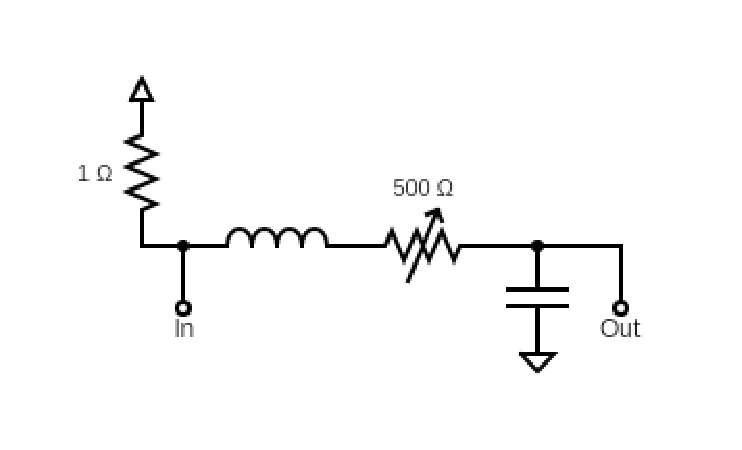
\includegraphics[width=4in]{circuit}
    \caption{The LRC circuit used in the second part of this lab (https://www.circuit-diagram.org/editor/)}
    \label{fig:circuit}
    \end{figure}
   
    The same four methods applied to measure the response function of the LRC circuit were also applied to an acoustical cavity. The acoustical cavity was set up so that a speaker pushed the sound into the bottom of the cylindrical container, and a microphone picked up the volume of the output on the top of the container. The microphone was plugged into the Teach Spin Fourier Methods Electronic Modules system and then fed into the appropriate analysis device; oscilloscope, lock-in amplifier, spectrum analyzer, or arduino system. The acoustical cavity had four possible heights: 3cm, 4cm, 5cm, and 6cm. Each of the four were analyzed. 
    
    Tubes have resonance frequencies where the nodes of the sound waves fit well in the tube. If the tubes don't have a wavelength that allows a node to find purchase on the opposite wall, some of the returning waves will destructively interfere with those coming from the speaker. However, when a resonance frequency is achieved, a sharp jump in the surviving amplitude can be observed. Similarly, when nearly all the reflected waves destructively interfere, the amplitude should drop to nearly zero. 
    
    For the first measurement method, measurements were taken from 1.3kHz to 4.3kHz with a step size of 0.3kHz. The noise drive was again used for the second method. The third method swept over a frequency of 0kHz (this was an option available for the Arduino, however it is hard to decipher what this data point actually means) to 10kHz with a step size of 500Hz and a drive amplitude of 0.95V. There were two sweeps taken to average the results. The same method to measure the transient response was used. 
    
    To save some time, only the 6cm cavity was used to measure the first method. The second and fourth methods used all four cavity sizes. Data was taken for the third method in all three cavity sizes; however, the data for the 3cm cavity was somehow lost in the process and will be excluded from the analysis.
    
    
    %% Results and Analysis section. Here I go into what we actually got out of the tests and the resulting calculations from them. 
    \section{Results and Analysis}
    
    This lab has been split up into the three different stages as explained above. The first outlines the first experiences with the spectrum analyzer and manually applying the FFT to the time domain in order to achieve the expected results. The second part goes over the LRC response function. The third goes over the acoustical cavity response function. 
    
    \subsection{General Fourier Introduction}
    It can be seen that the difference between the uniform window and hanning window in Figure~\ref{fig:1 sine uniform} and Figure~\ref{fig:1 sine hanning} isn't very noticeable. However, when applied to a frequency that wasn't as ideal, such as in Figure~\ref{fig:1.03 sine uniform} and Figure~\ref{fig:1.03 sine hanning}, the hanning correction made the FFT of the 1.03kHz frequency (Figure~\ref{fig:1.03 sine hanning} look comparable to that of the 1kHz frequency (Figure~\ref{fig:1 sine uniform}. 
    
    \begin{figure}[!ht]
        \centering
        \begin{subfigure}[h]{\textwidth}
        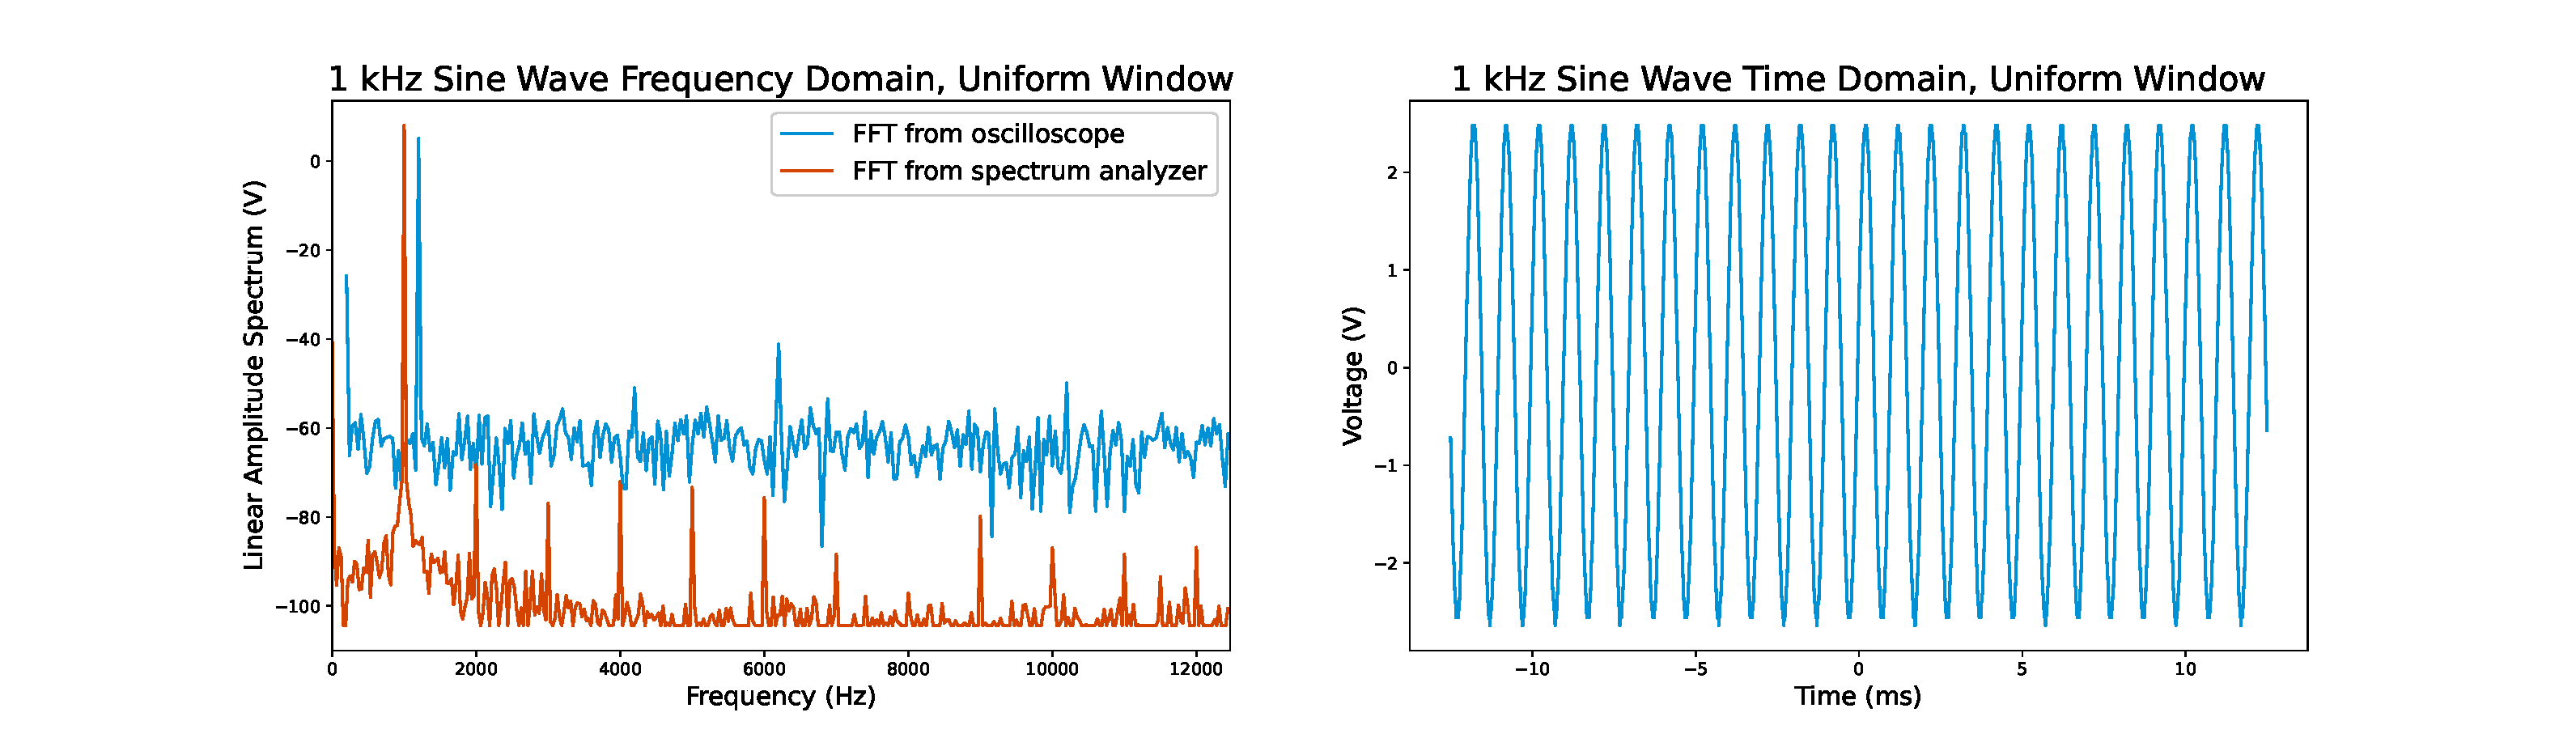
\includegraphics[width=\textwidth]{1 kHz Sine Wave (uniform)}
        \caption{}
        \label{fig:1 sine uniform}
        \end{subfigure}
        \begin{subfigure}[h]{\textwidth}
        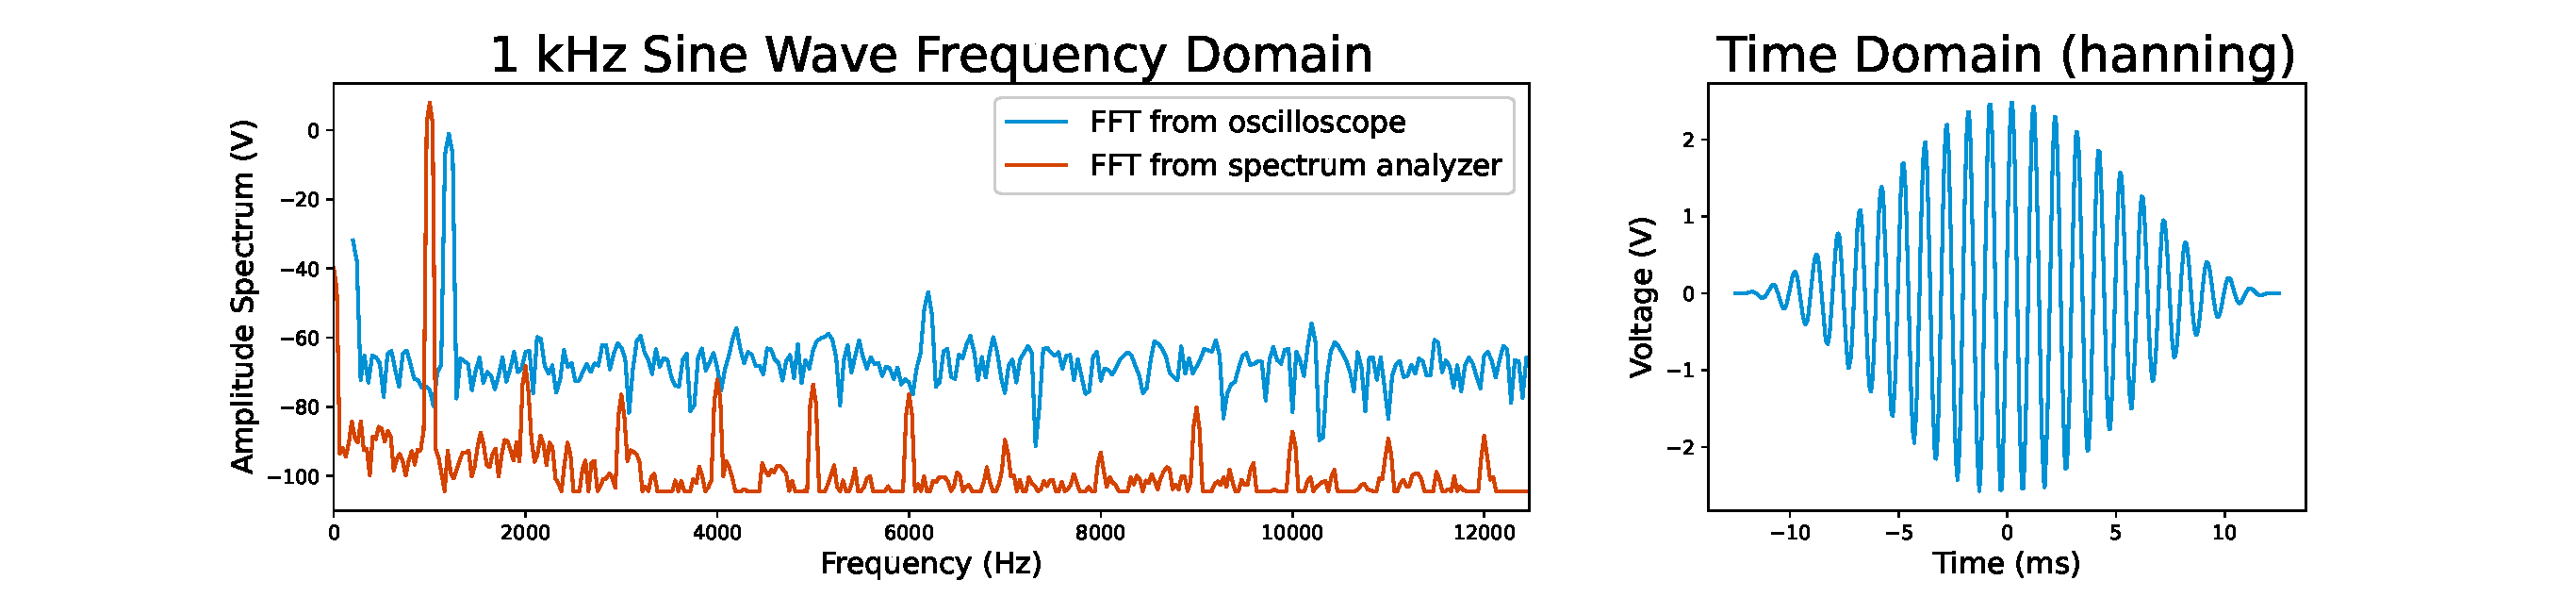
\includegraphics[width=\textwidth]{1 kHz Sine Wave (hanning)}
        \caption{}
        \label{fig:1 sine hanning}
        \end{subfigure}
        \begin{subfigure}[h]{\textwidth}
        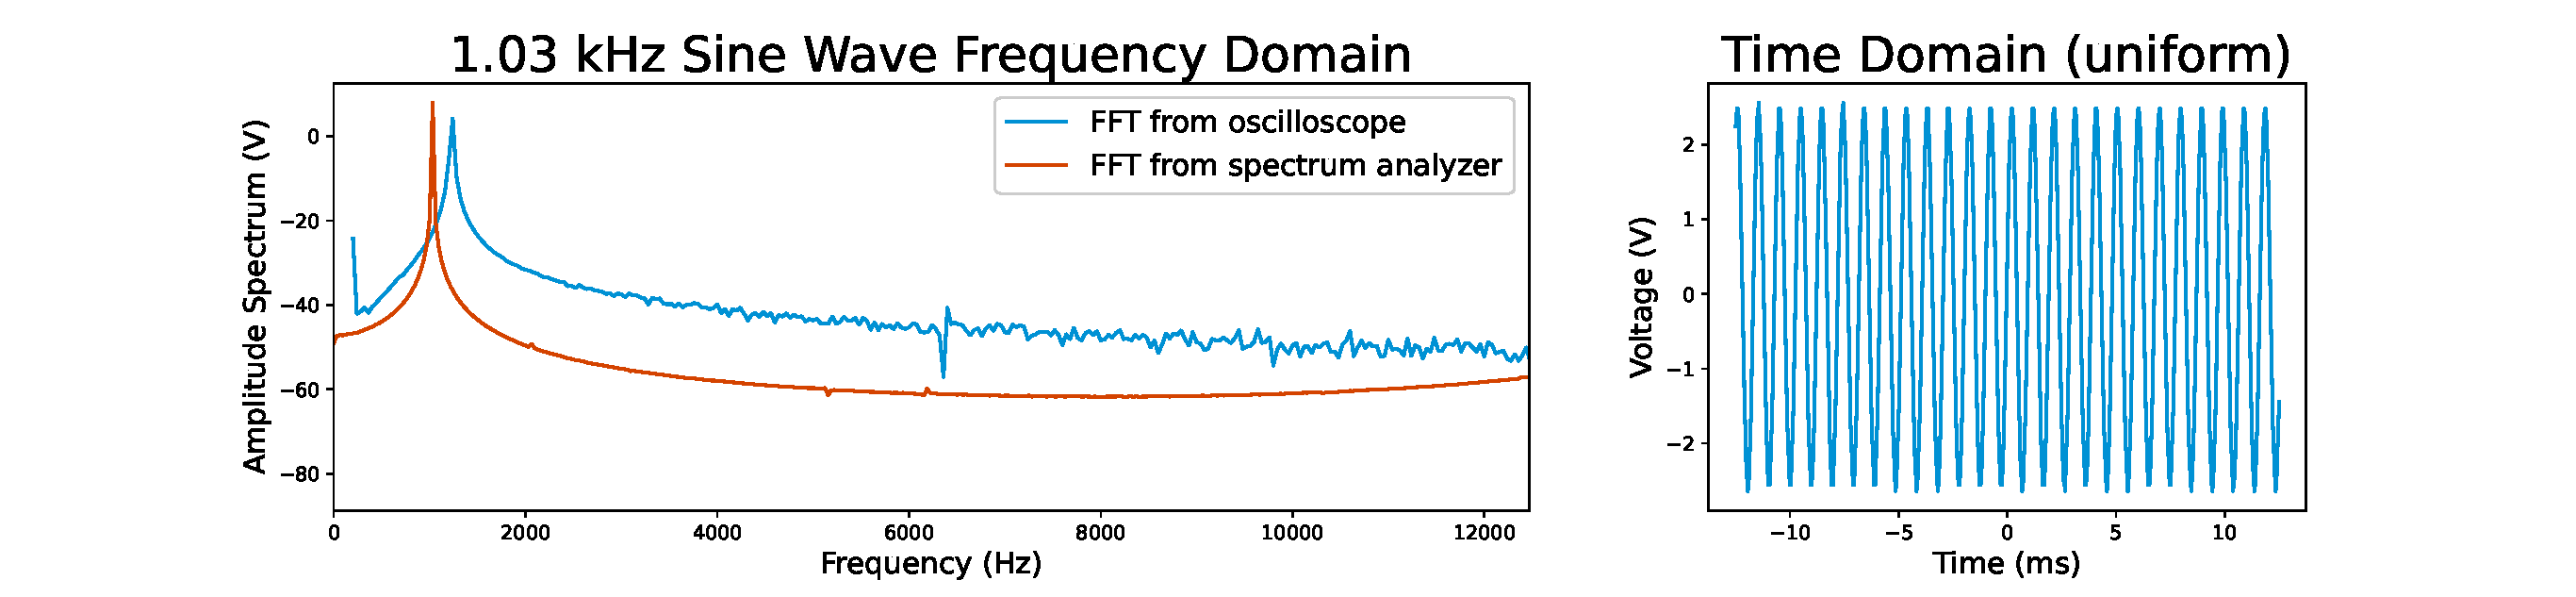
\includegraphics[width=\textwidth]{1_03 kHz Sine Wave (uniform)}
        \caption{}
        \label{fig:1.03 sine uniform}
        \end{subfigure}
        \begin{subfigure}[h]{\textwidth}
        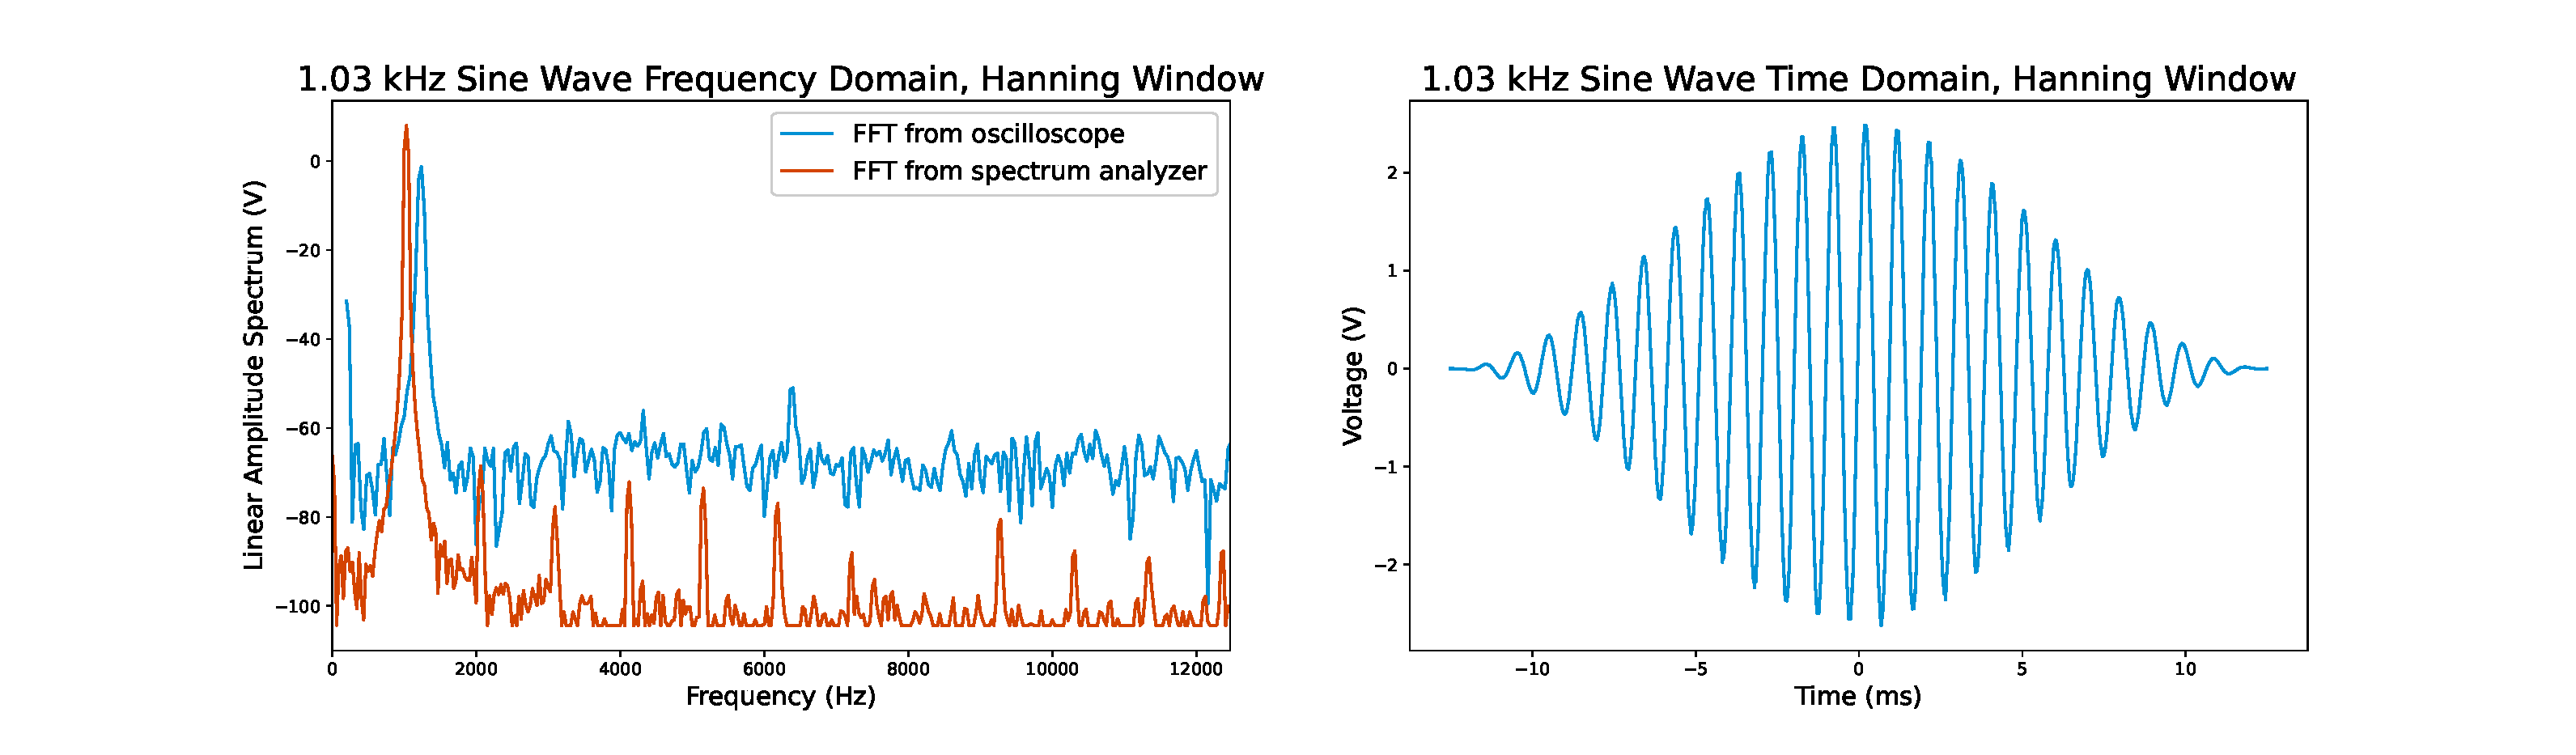
\includegraphics[width=\textwidth]{1_03 kHz Sine Wave (hanning)}
        \caption{}
        \label{fig:1.03 sine hanning}
        \end{subfigure}
    \end{figure} % Sine Waves
    
    \begin{figure}[!ht]
        \centering
        \begin{subfigure}[h]{\textwidth}
        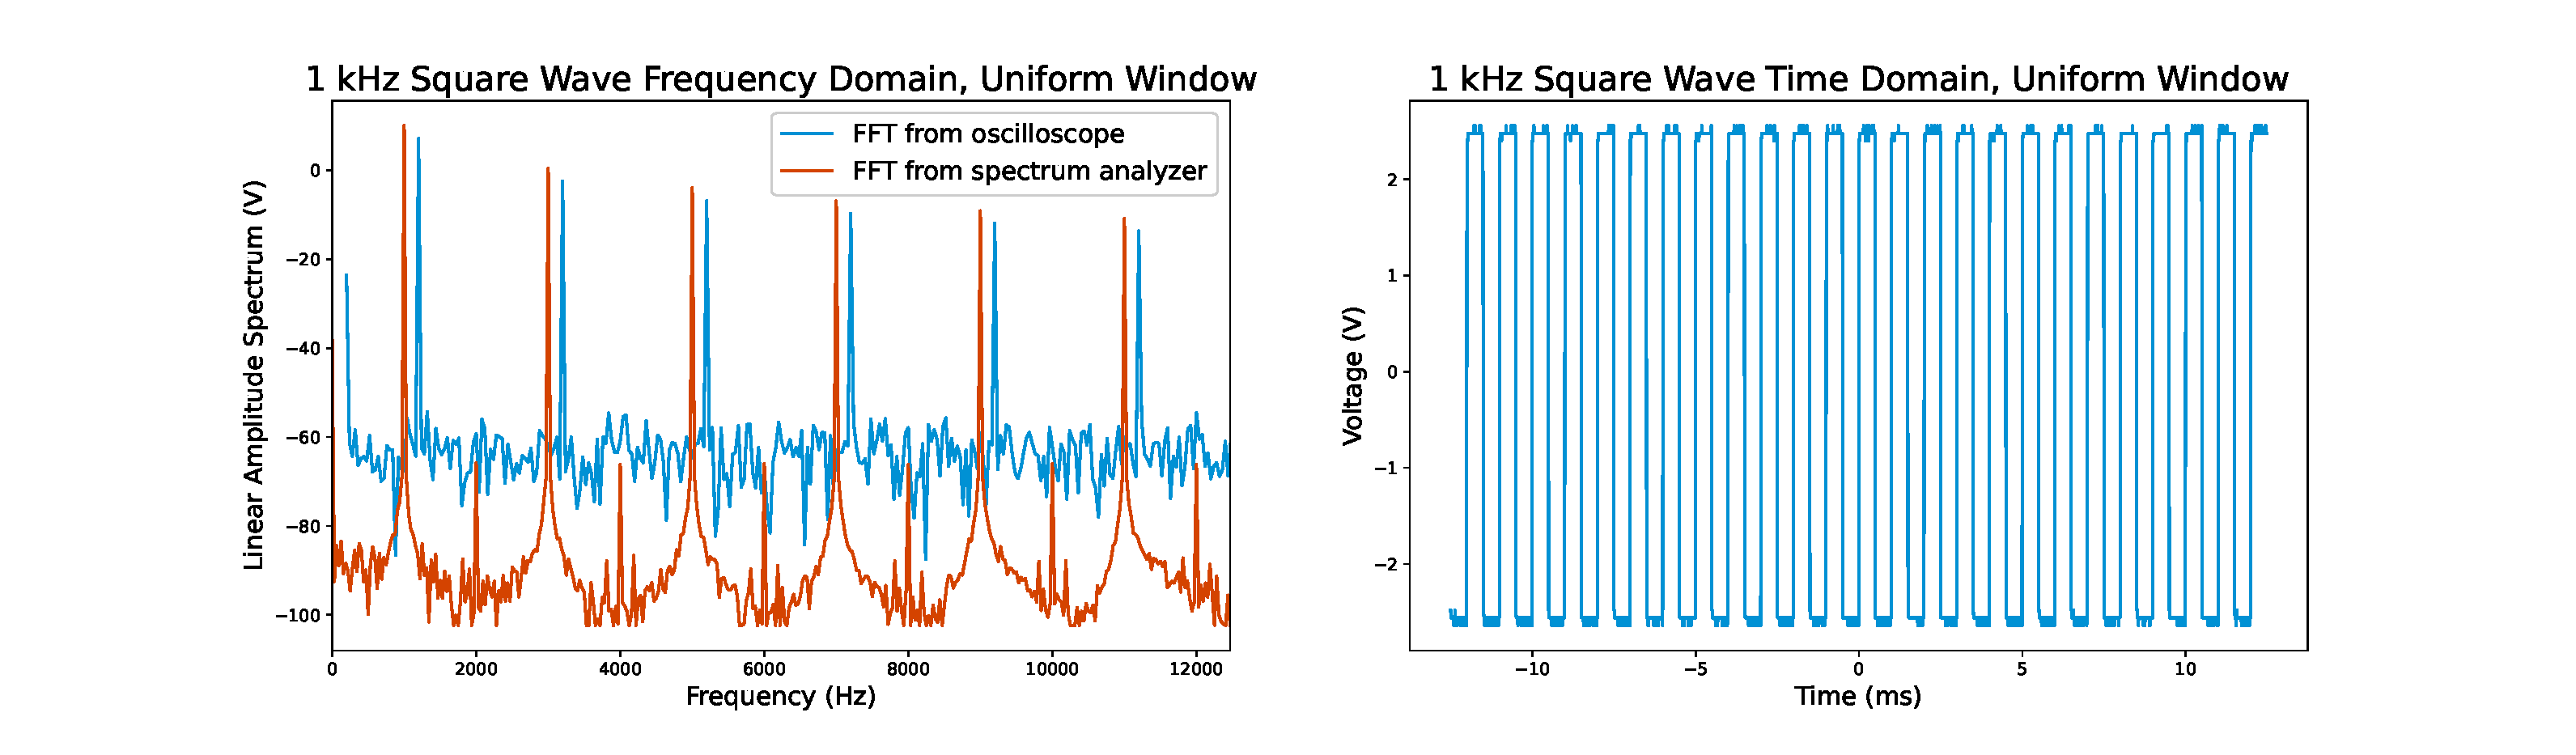
\includegraphics[width=\textwidth]{1 kHz Square Wave (uniform)}
        \caption{}
        \label{fig:1 square uniform}
        \end{subfigure}
        \begin{subfigure}[h]{\textwidth}
        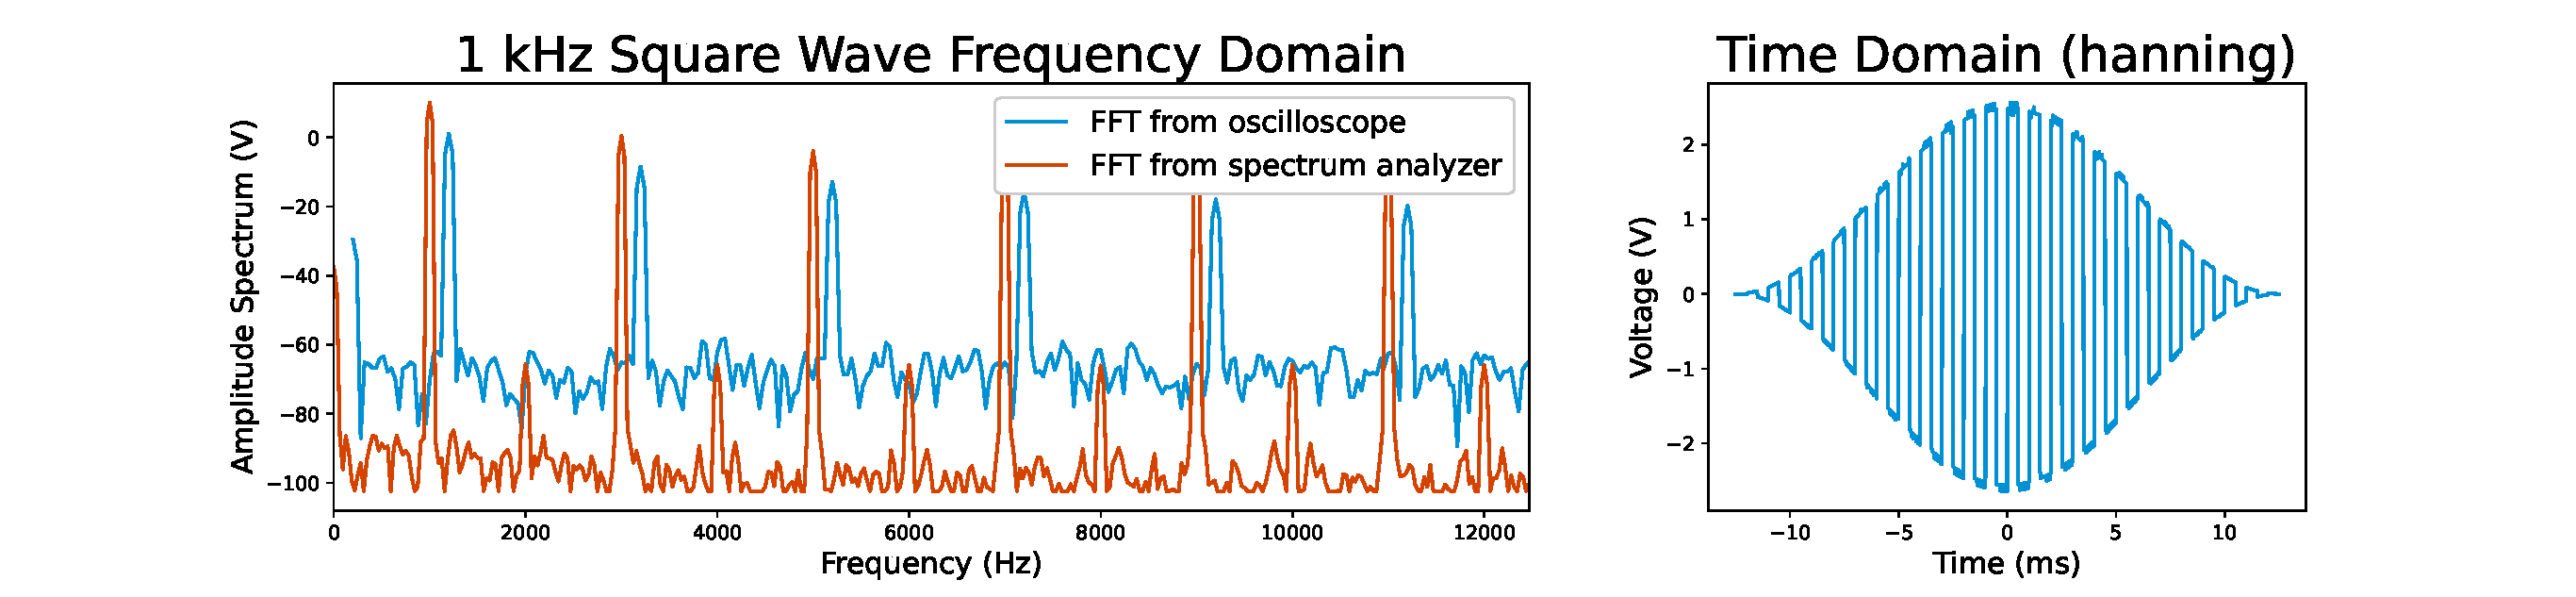
\includegraphics[width=\textwidth]{1 kHz Square Wave (hanning)}
        \caption{}
        \label{fig:1 square hanning}
        \end{subfigure}
        \begin{subfigure}[h]{\textwidth}
        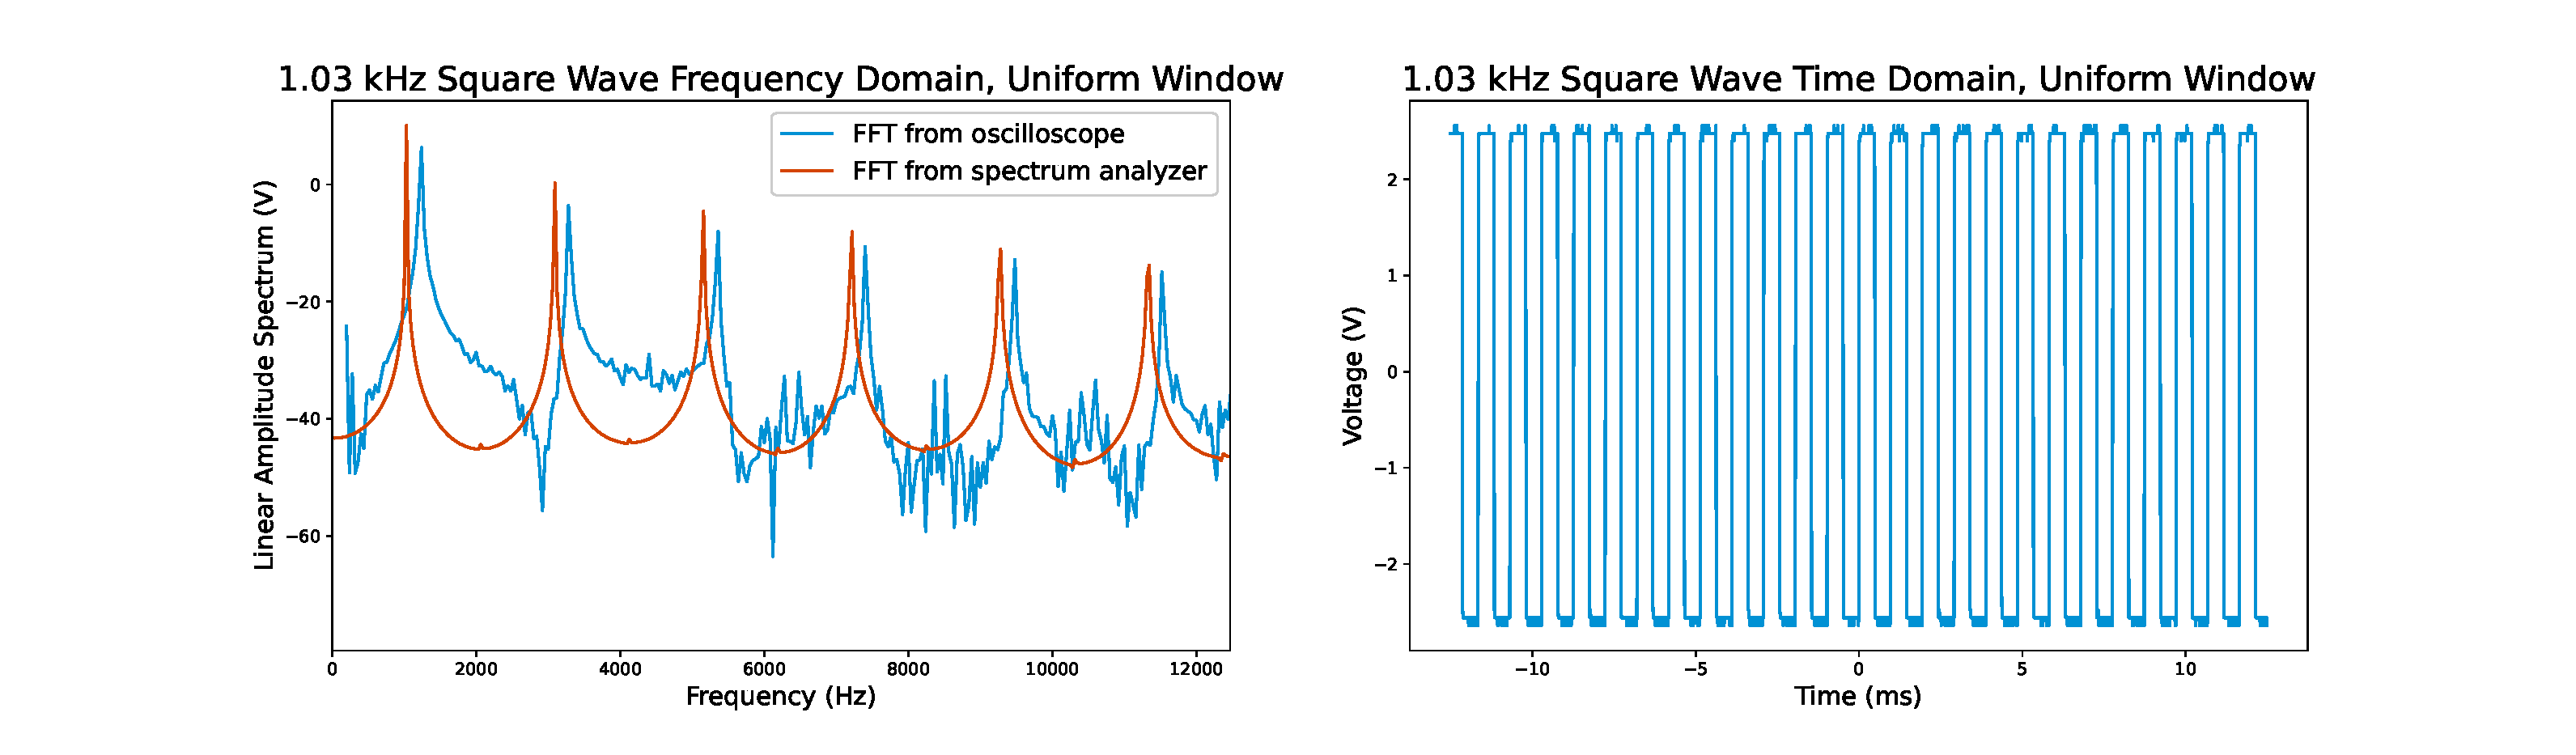
\includegraphics[width=\textwidth]{1_03 kHz Square Wave (uniform)}
        \caption{}
        \label{fig:1.03 square uniform}
        \end{subfigure}
        \begin{subfigure}[h]{\textwidth}
        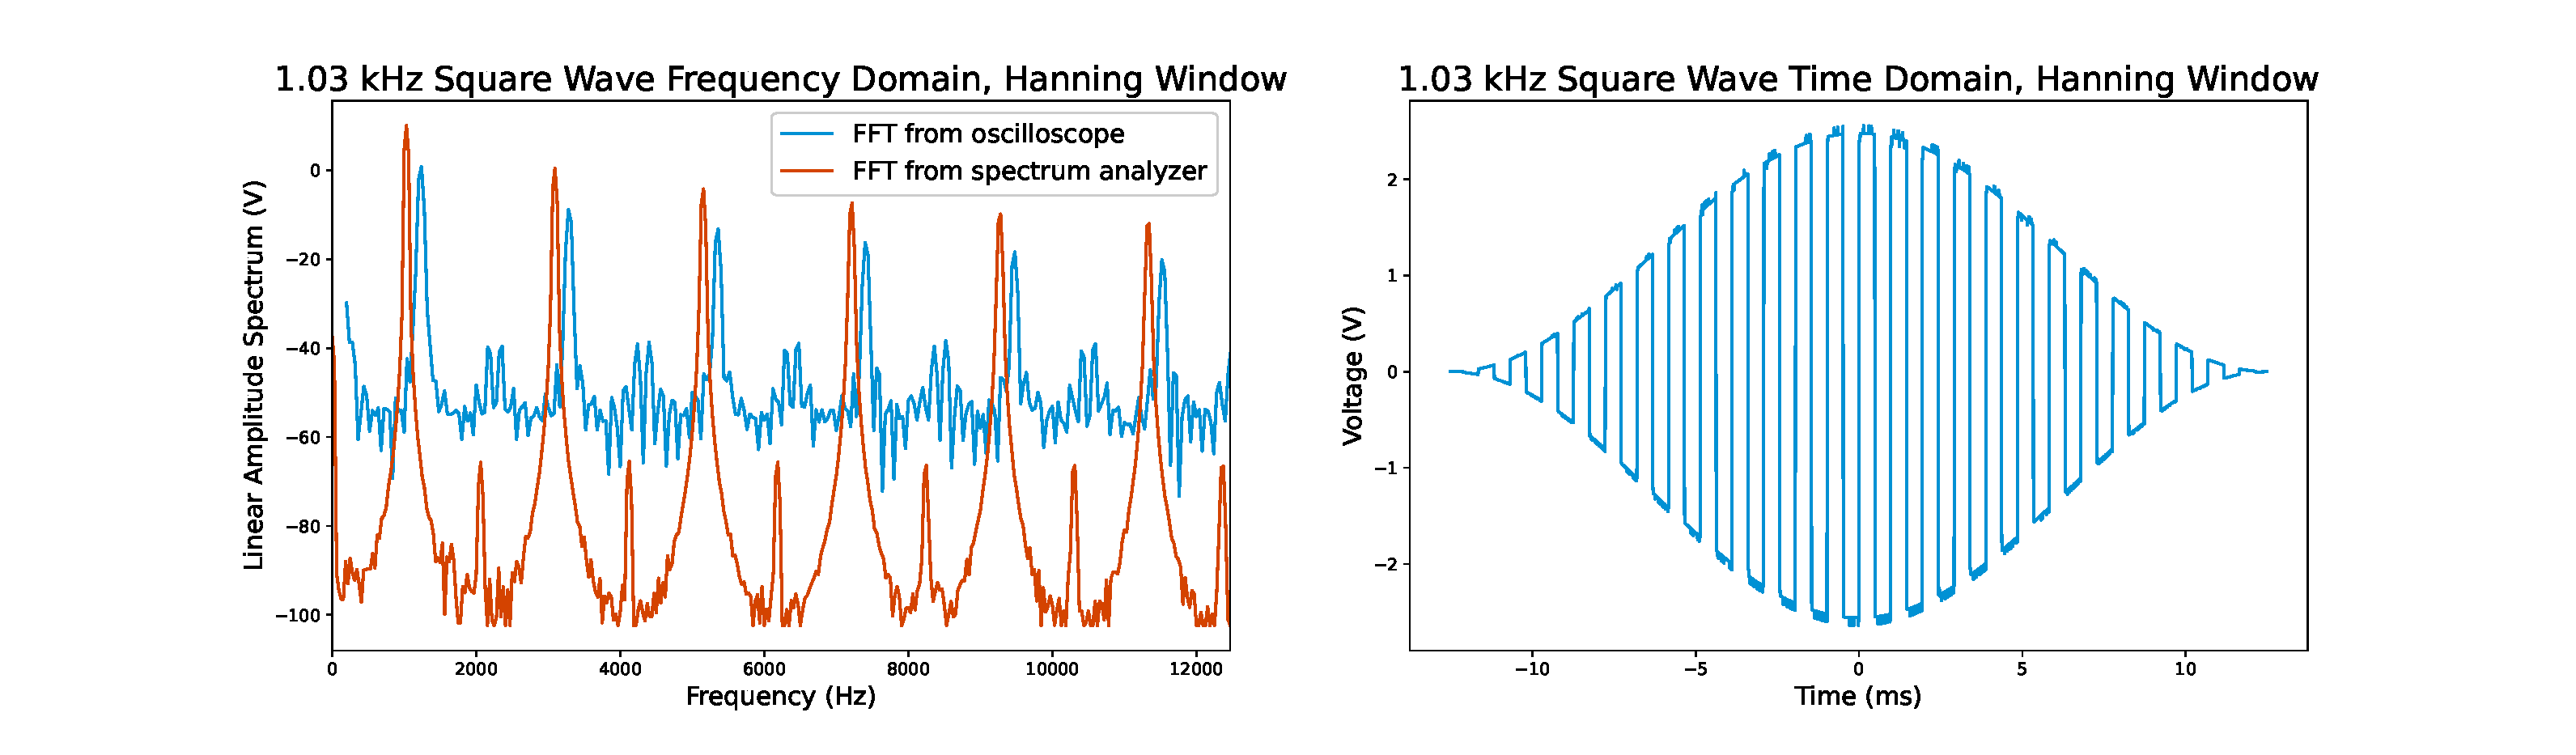
\includegraphics[width=\textwidth]{1_03 kHz Square Wave (hanning)}
        \caption{}
        \label{fig:1.03 square hanning}
        \end{subfigure}
    \end{figure} % Square Waves
    
    \begin{figure}[!ht]
        \centering
        \begin{subfigure}[h]{\textwidth}
        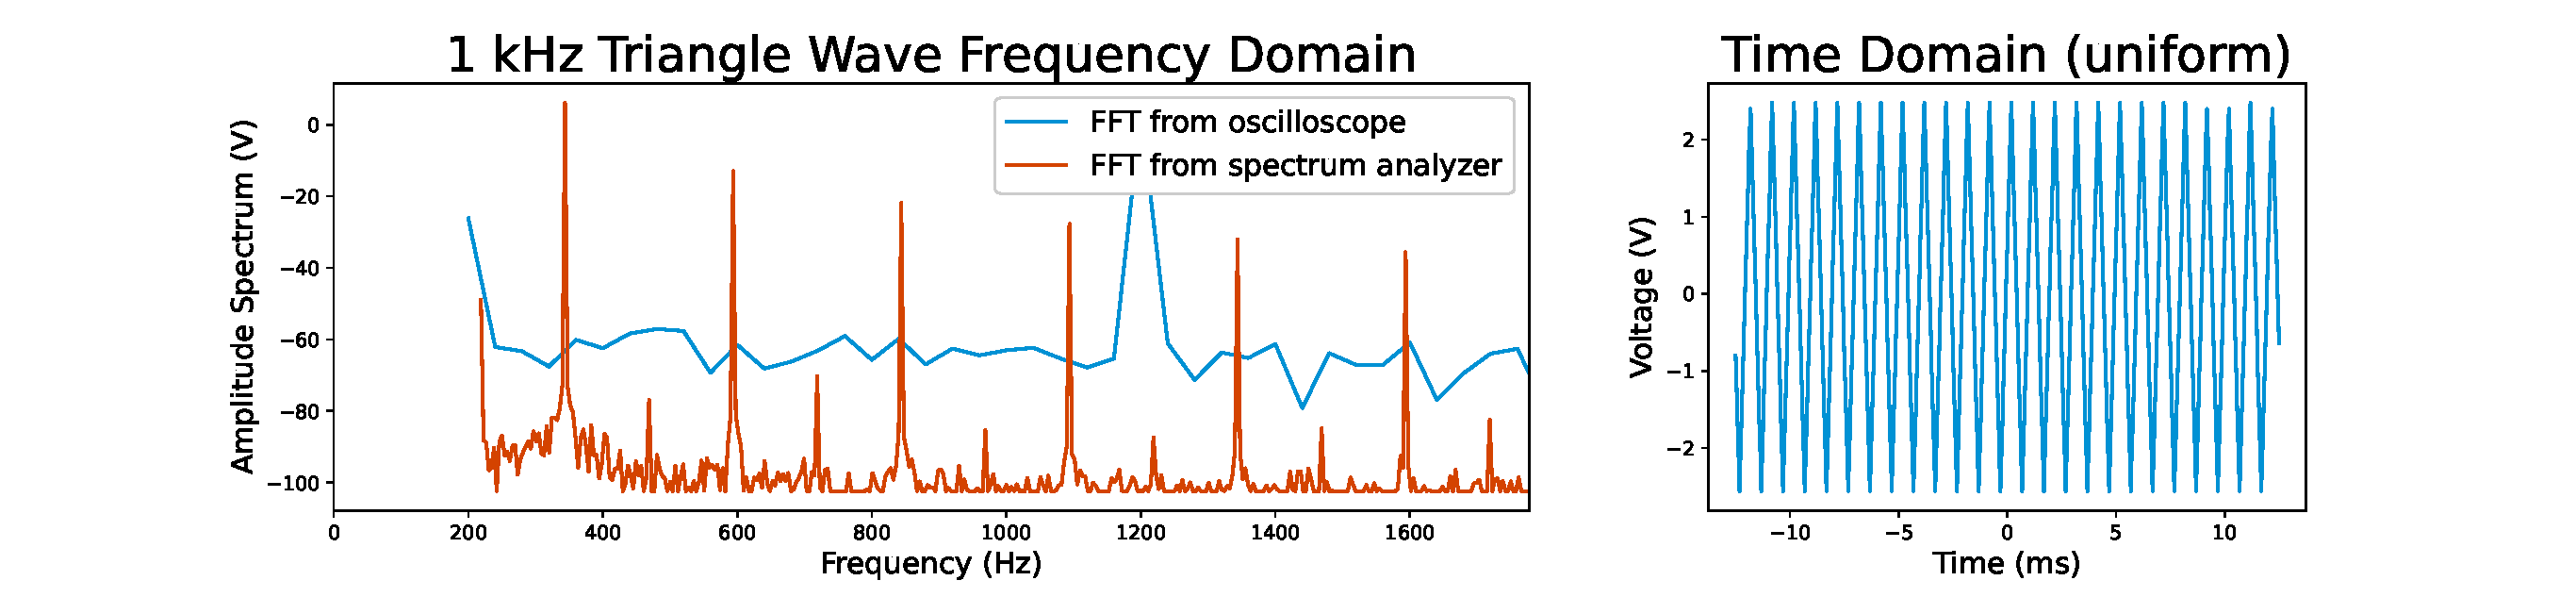
\includegraphics[width=\textwidth]{1 kHz Triangle Wave (uniform)}
        \caption{}
        \label{fig:1 triangle uniform}
        \end{subfigure}
        \begin{subfigure}[h]{\textwidth}
        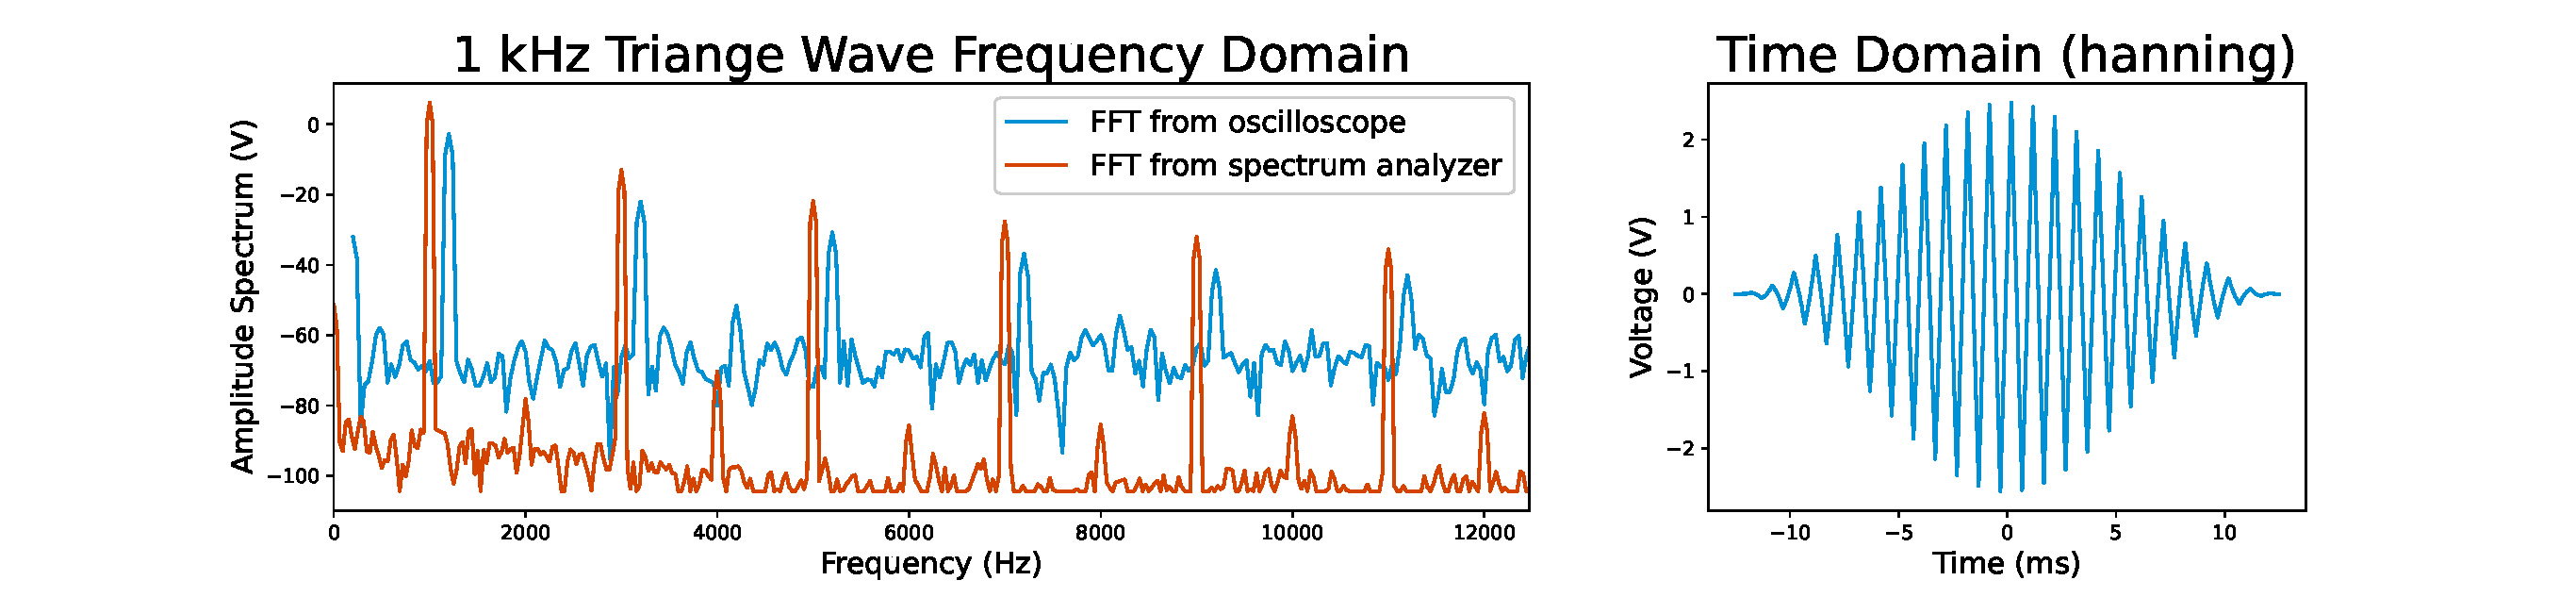
\includegraphics[width=\textwidth]{1 kHz Triange Wave (hanning)}
        \caption{}
        \label{fig:1 triangle hanning}
        \end{subfigure}
        \begin{subfigure}[h]{\textwidth}
        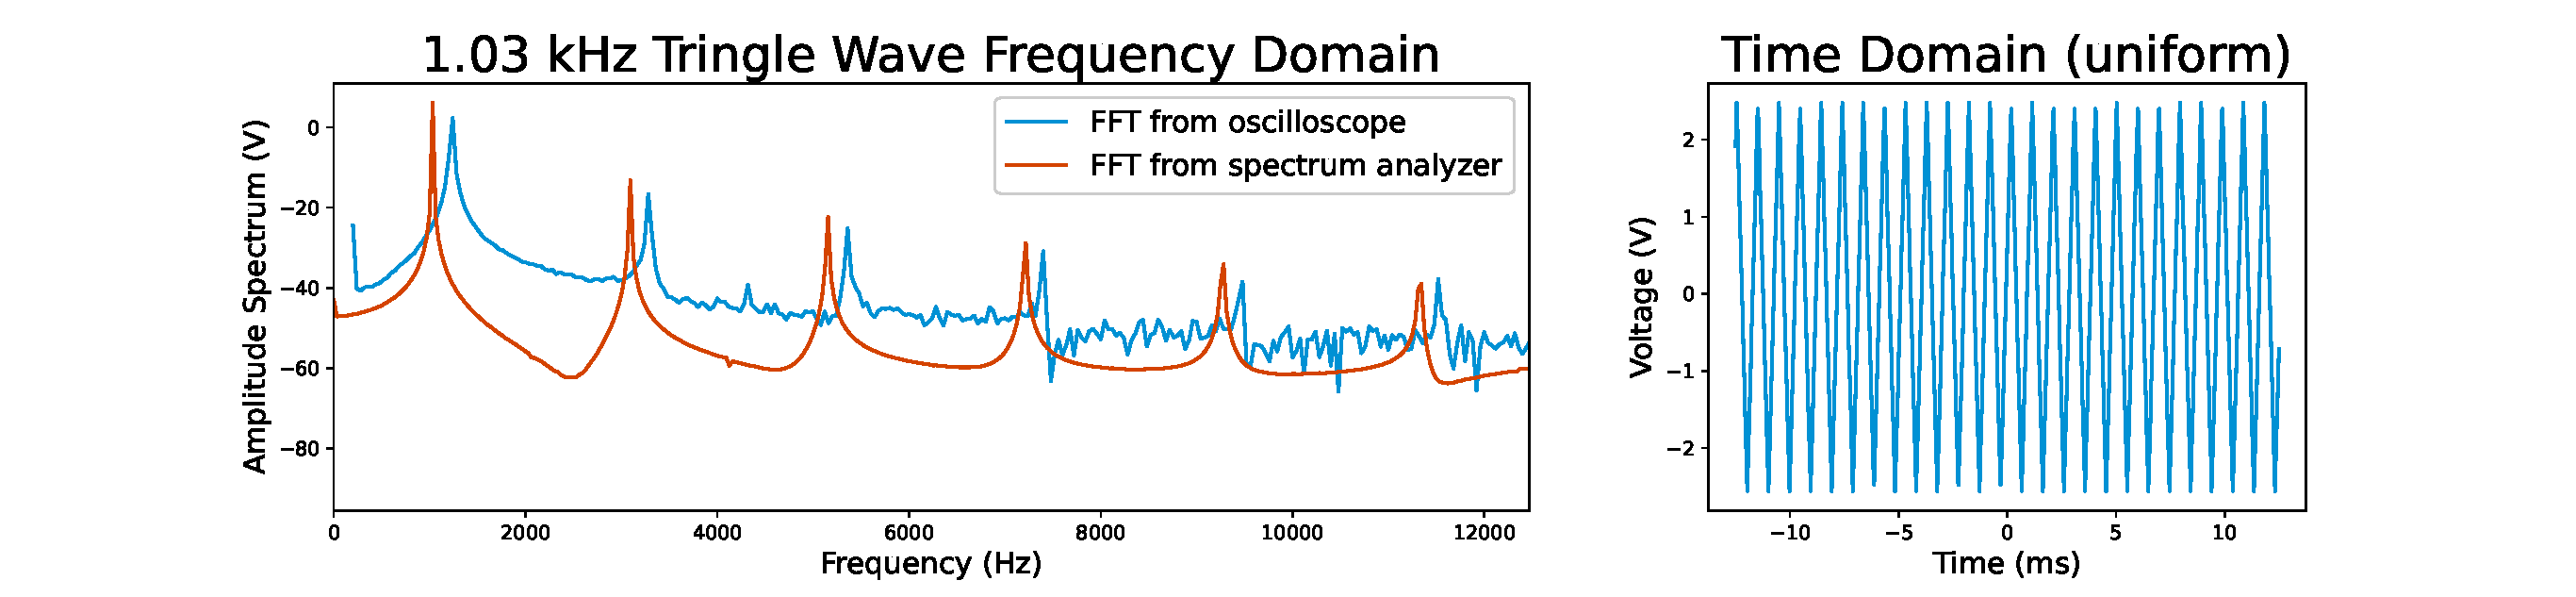
\includegraphics[width=\textwidth]{1_03 kHz Tringle Wave (uniform)}
        \caption{}
        \label{fig:1.03 triangle uniform}
        \end{subfigure}
        \begin{subfigure}[h]{\textwidth}
        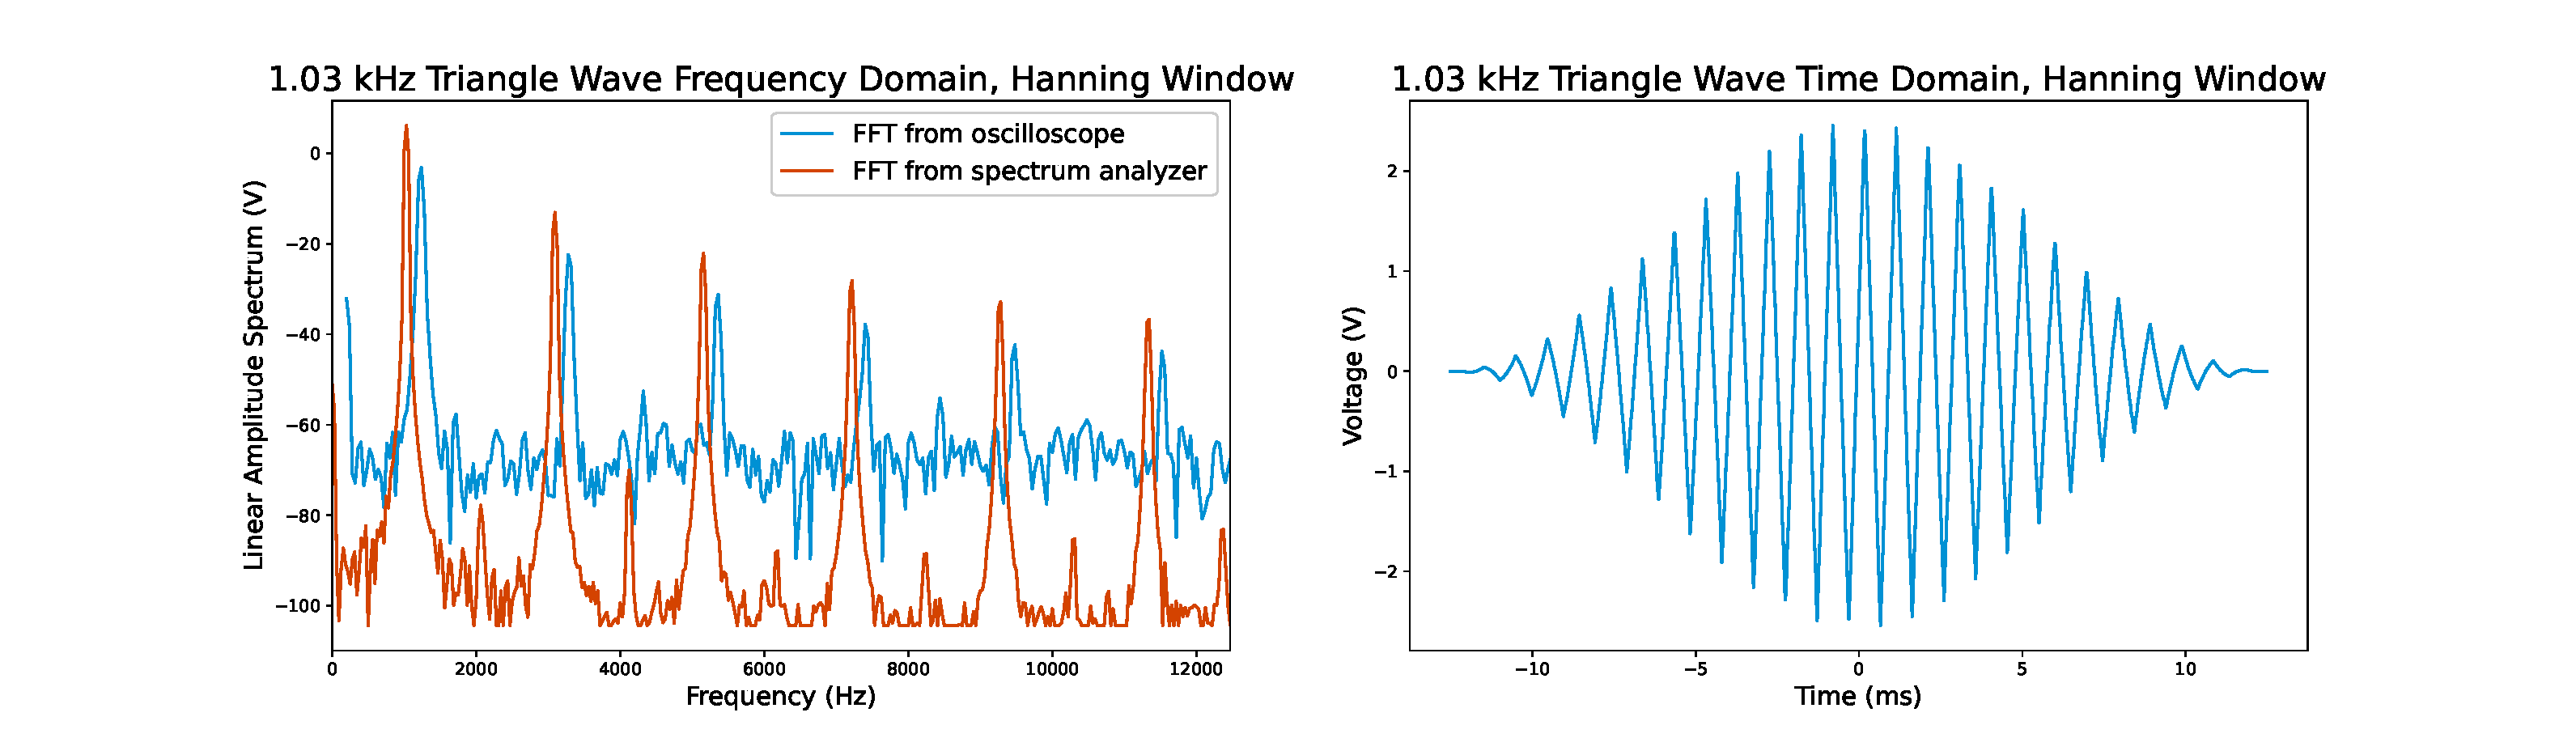
\includegraphics[width=\textwidth]{1_03 kHz Triangle Wave (hanning)}
        \caption{}
        \label{fig:1.03 triangle hanning}
        \end{subfigure}
    \end{figure} % Triangle Waves
    
    It seems that using the hanning window on anything, other than the ideal Sine Wave, returned a more reasonable analysis; for both the spectrum analyzer and the oscilloscope. It can be seen that the FFT of the less ideal frequency has a wider spread of possible frequency peak. This should serve as the practical average and standard deviation of the result; taking the highest peak as the average and the HMFW to be the standard deviation.
    
    To test the impact of different windows on the FFT, five different windows were tested on a square wave (Figure~\ref{fig:various windows}. While this doesn't give any enlightenment as to where each shines, the largest take away is that the four window functions that are not the uniform window effectively grounded the noise introduced to the FFT by a non-periodic function.  
    
    \begin{figure}[!ht]
        \centering
        \begin{subfigure}[h]{\textwidth}
        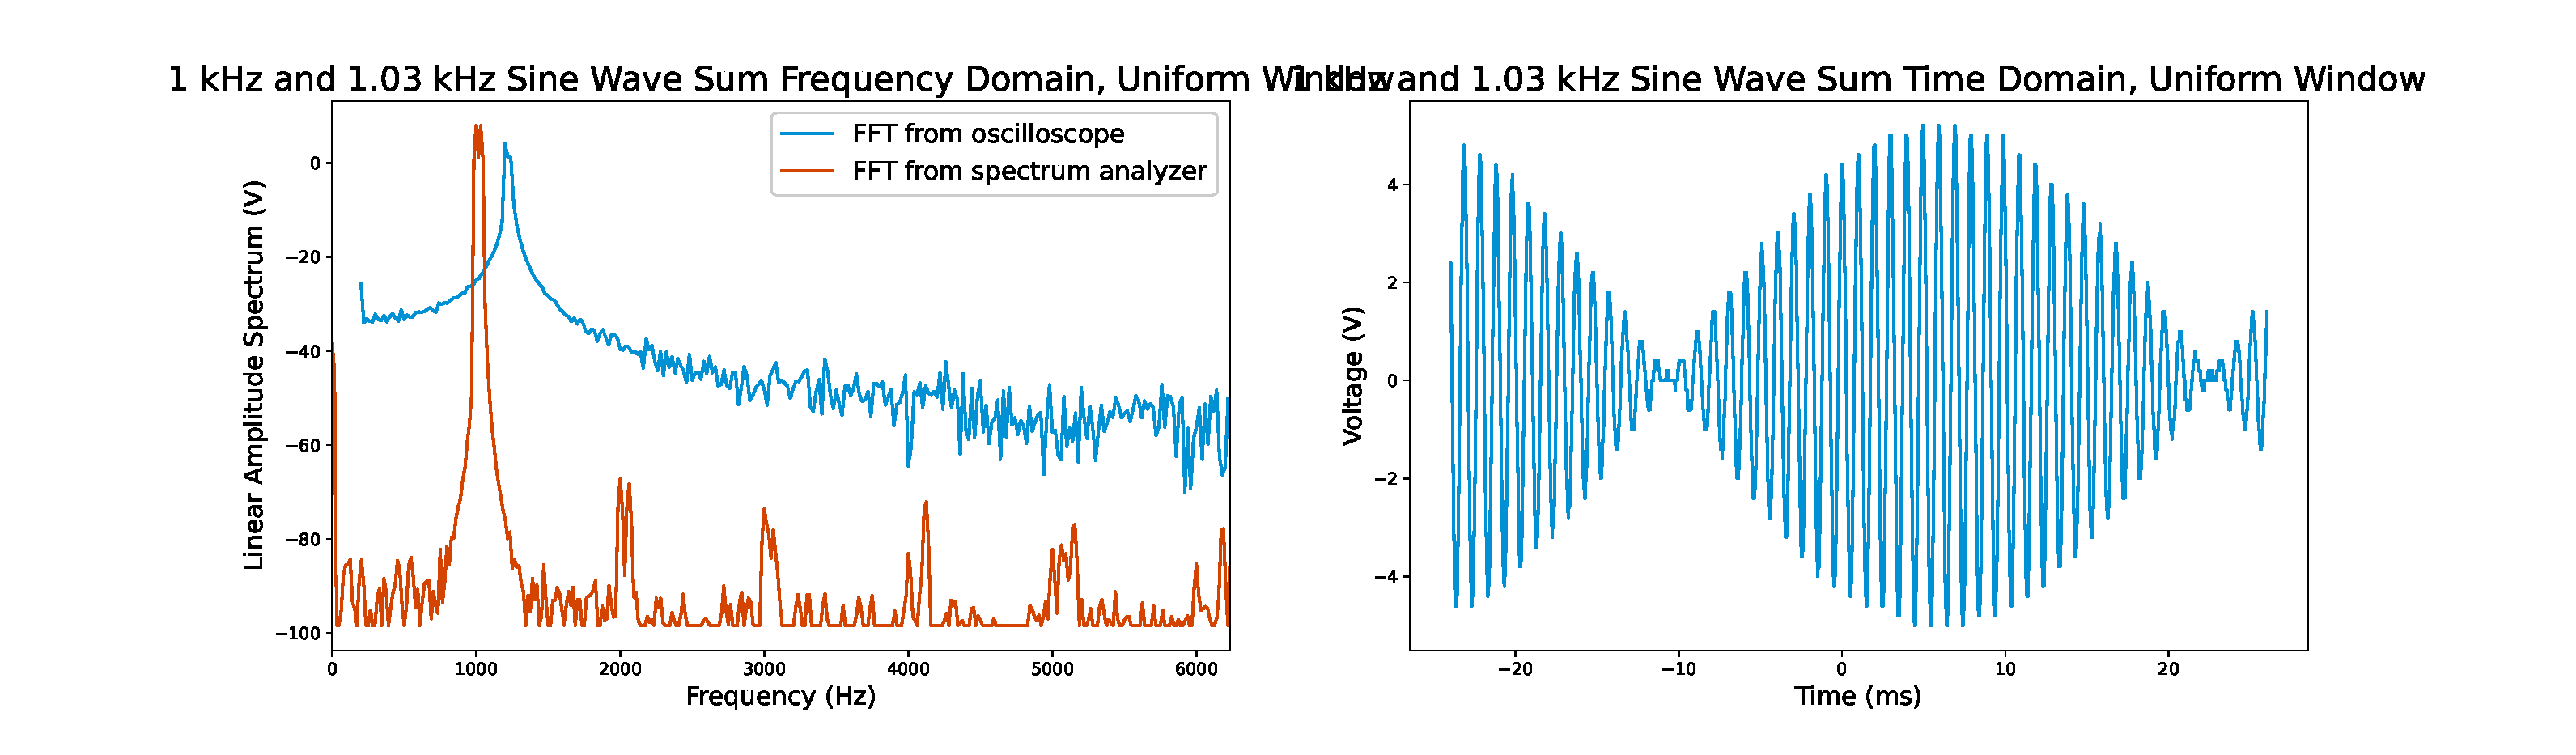
\includegraphics[width=\textwidth]{1 kHz and 1_03 kHz Sine Wave Sum (uniform)}
        \caption{}
        \label{fig:sine sum}
        \end{subfigure}
        \begin{subfigure}[h]{\textwidth}
        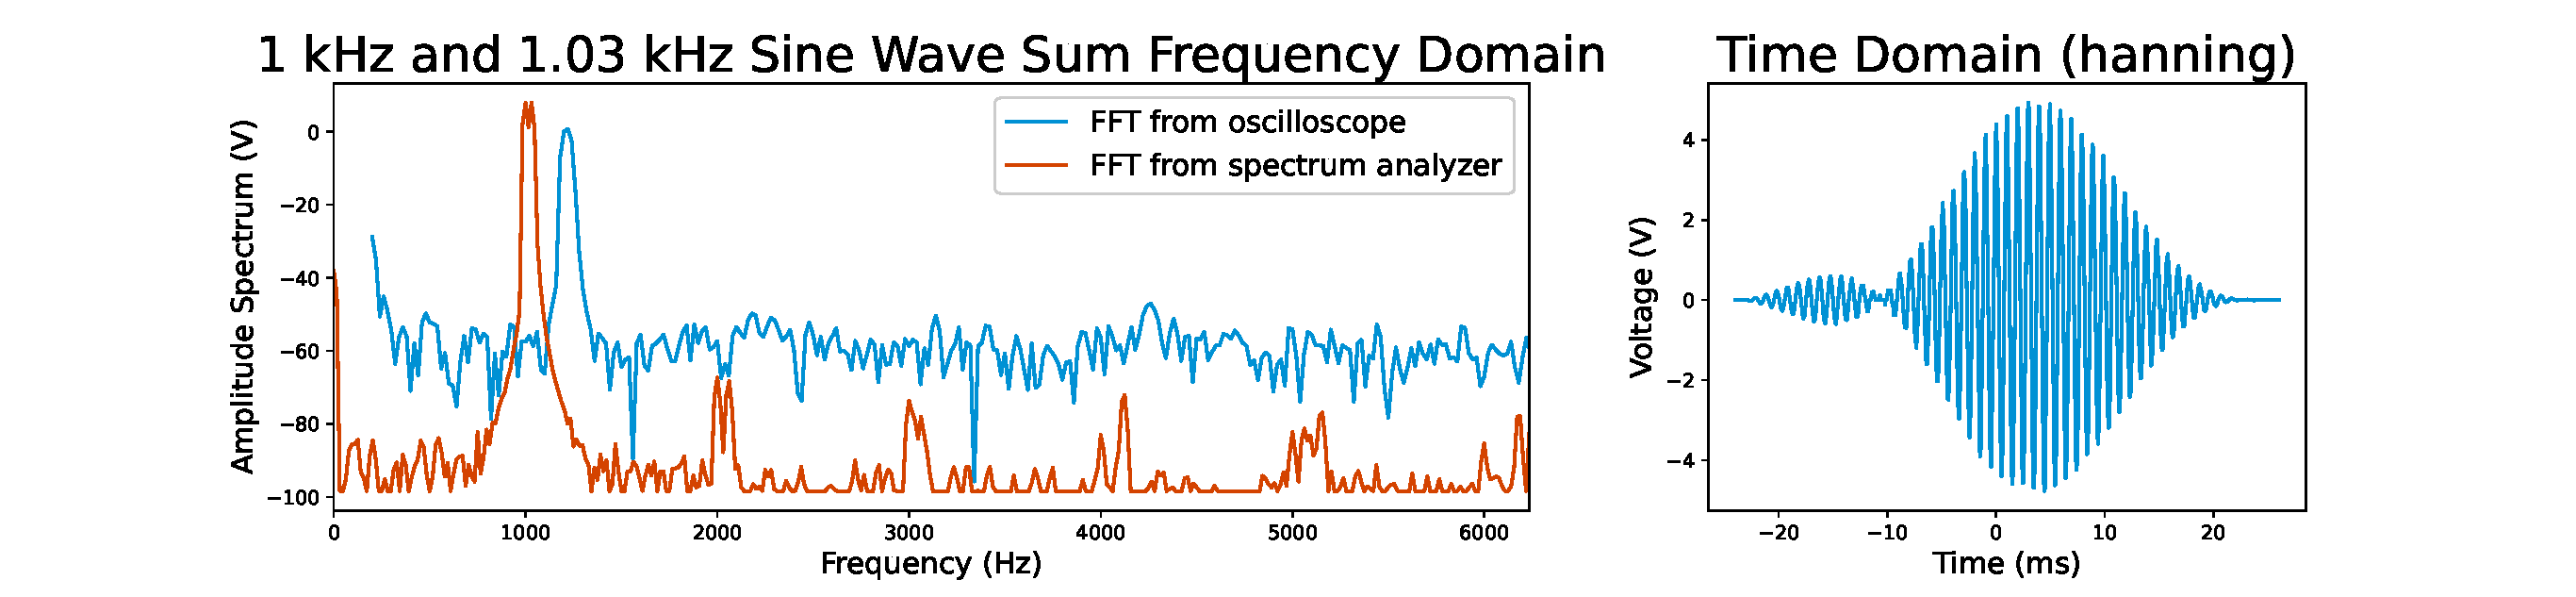
\includegraphics[width=\textwidth]{1 kHz and 1_03 kHz Sine Wave Sum (hanning)}
        \caption{}
        \label{fig:sine sum}
        \end{subfigure}
    \end{figure} % sum
    
    \begin{figure}[!ht]
        \centering
        \begin{subfigure}[h]{\textwidth}
        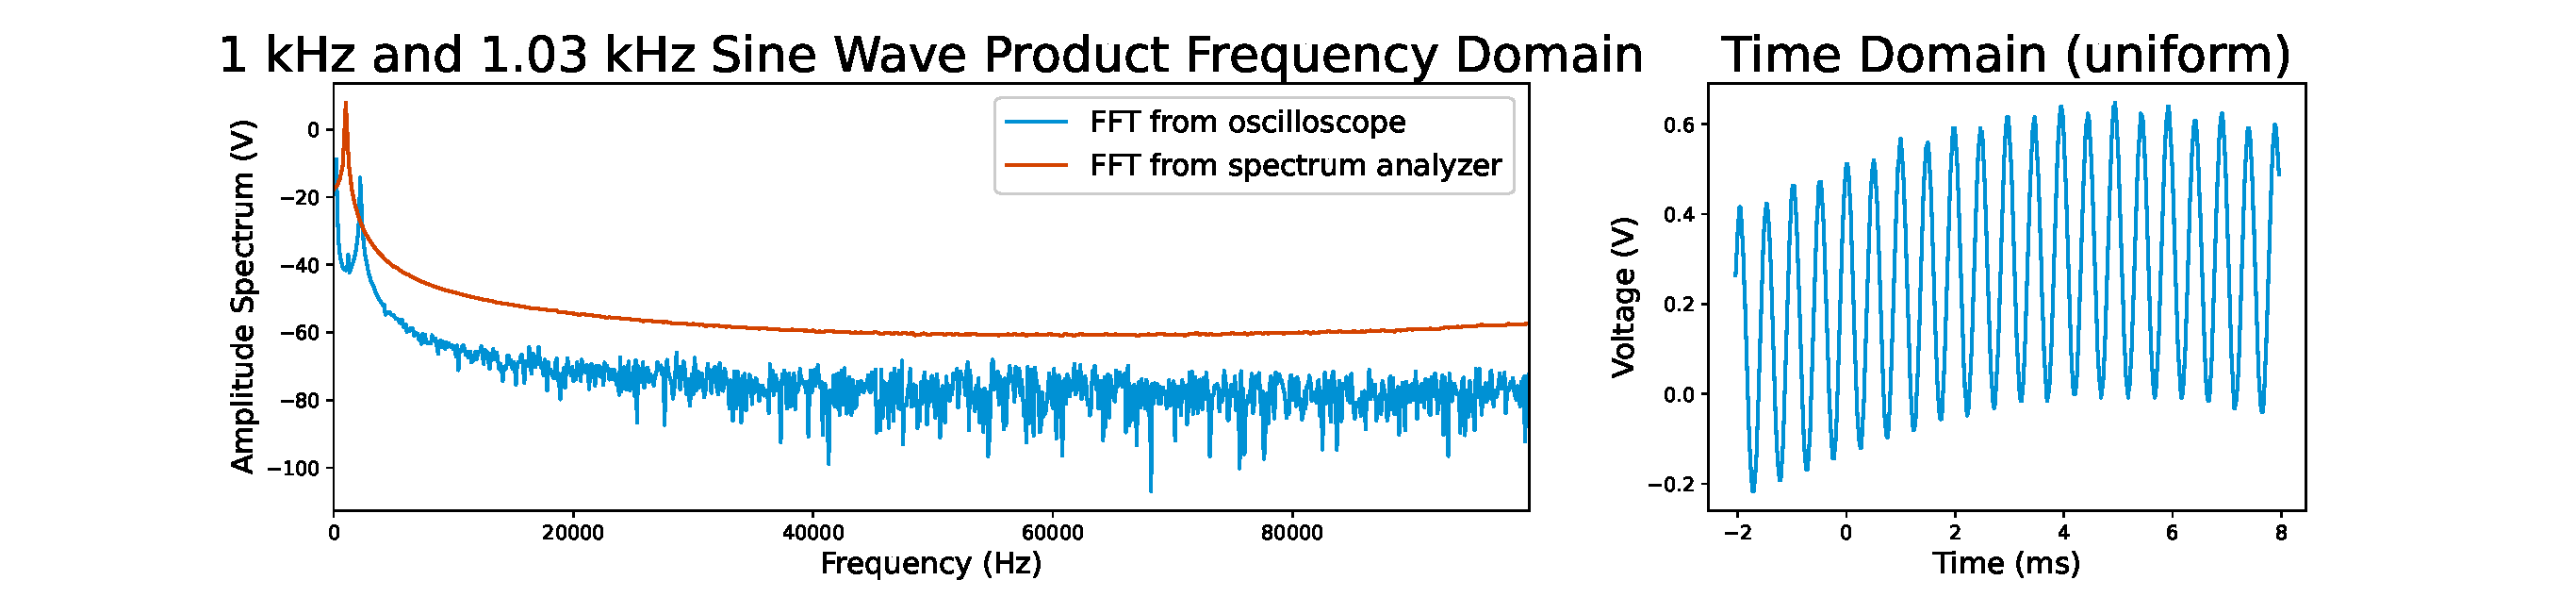
\includegraphics[width=\textwidth]{1 kHz and 1_03 kHz Sine Wave Product (uniform)}
        \caption{}
        \label{fig:sine product}
        \end{subfigure}
        \begin{subfigure}[h]{\textwidth}
        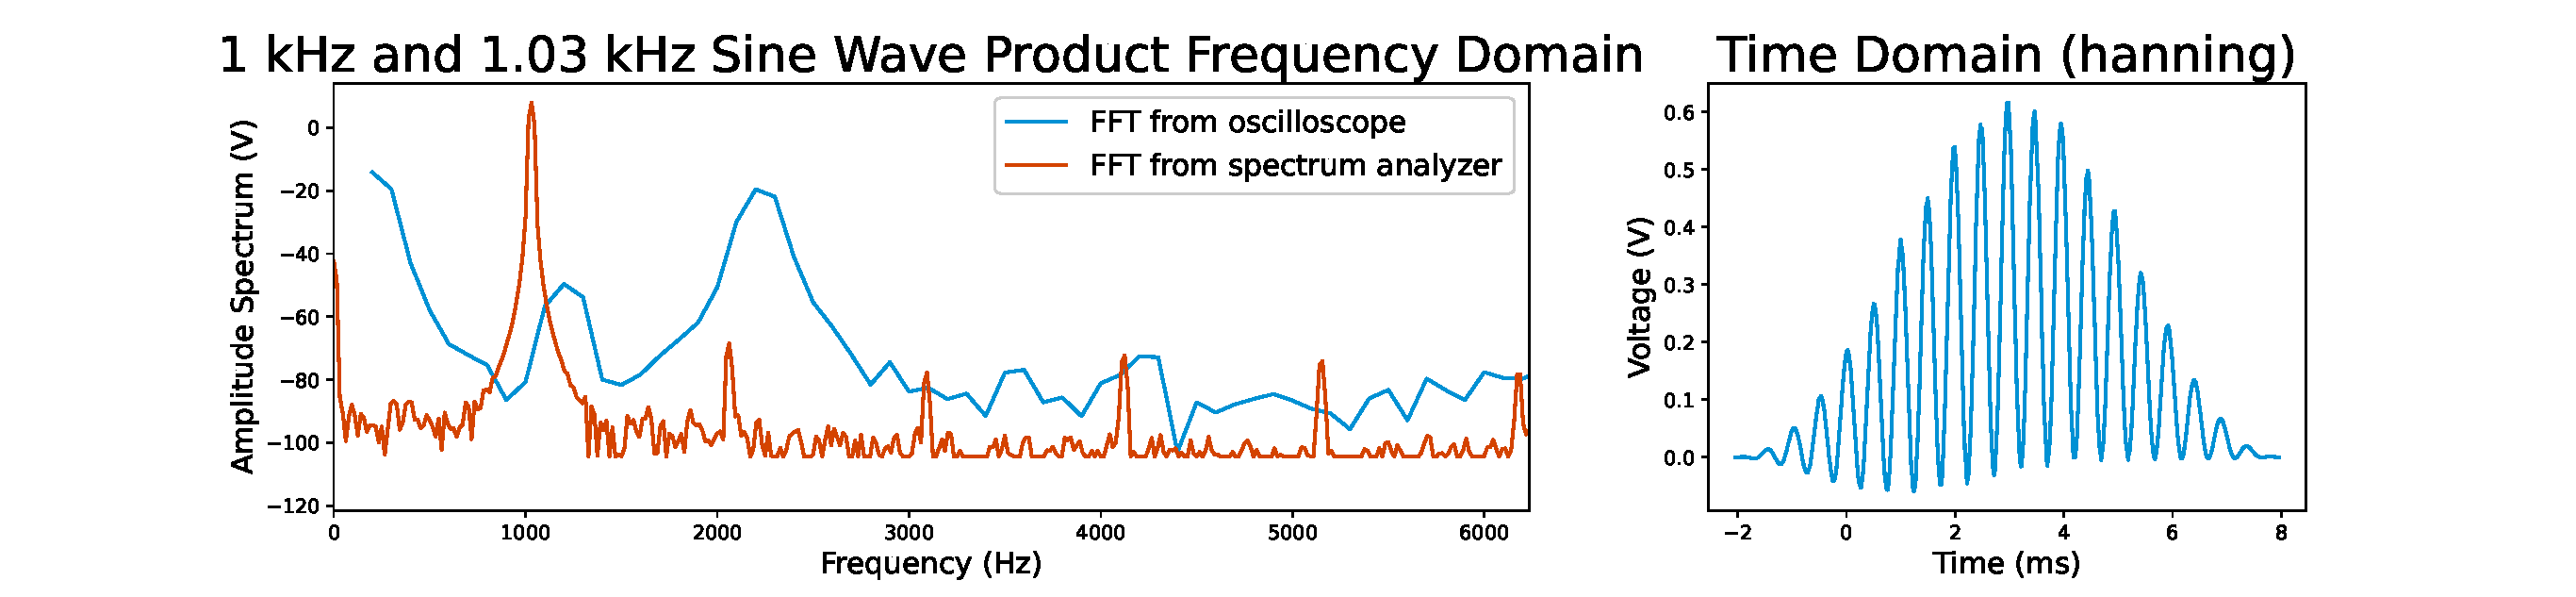
\includegraphics[width=\textwidth]{1 kHz and 1_03 kHz Sine Wave Product (hanning)}
        \caption{}
        \label{fig:sine product}
        \end{subfigure}
    \end{figure} % product
    
    \begin{figure}
    \centering
        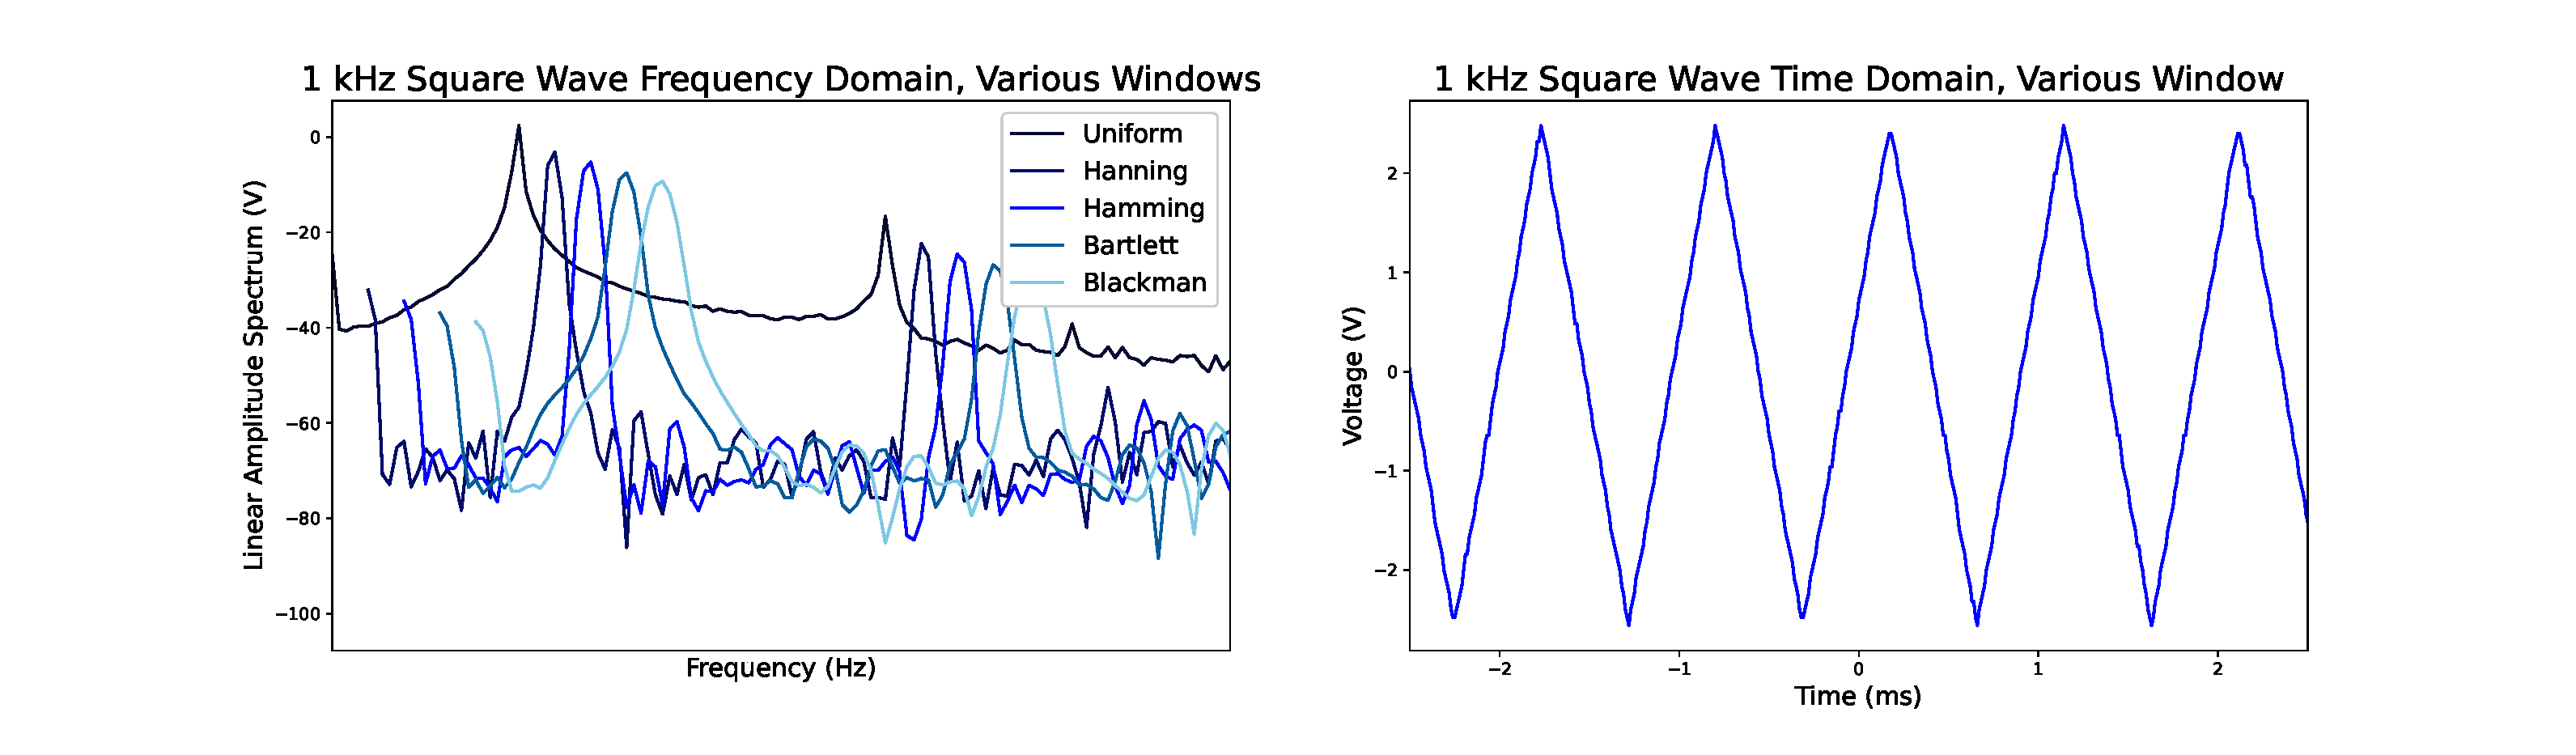
\includegraphics[width=\textwidth]{Variety of Windows}
        \caption{}
        \label{fig:various windows}
    \end{figure} % variety of windows
    
    The final test to see if we understood Fourier Analysis was to find the treasure buried in the noise provided. The tests were labeled A, B, C, and D. The first three were attempted, and only the first two could be found within the time restraint. On setting A, once the data was averaged over a large number of passes, about 1000, the spectrum analyzer seemed to give a definitive spike (Figure~\ref{fig:buried A}. The oscilloscope collected data with an acquire time about the same as that used for the spectrum analyzer, 32ms, and averaged over 128 passes. Even with the large amount of data collection, the peak is barely visible. On setting B (Figure~\ref{fig:buried B}), with even more passes averaged and an acquire time of 8ms, the specturm analyzer could barely pick out the peak and nothing was found from the FFT done post lab. On setting C (Figure~\ref{fig:buried C}), the noise was so dominant nothing was able to be picked out. 
    
    \begin{figure}[!ht]
        \centering
        \begin{subfigure}[h]{\textwidth}
        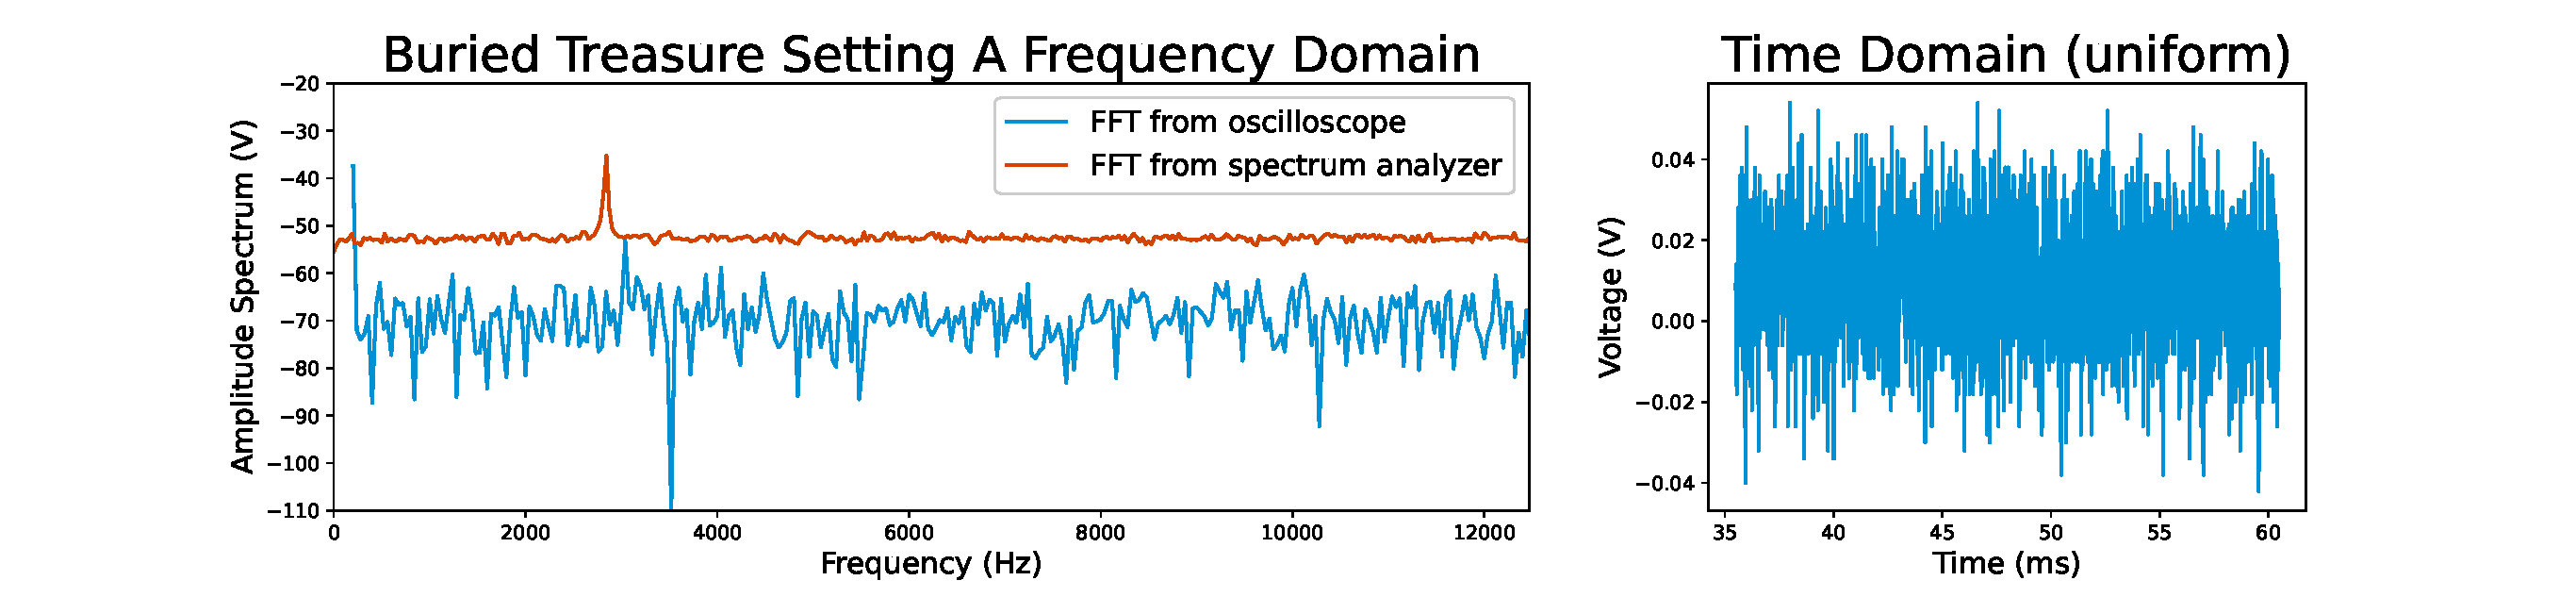
\includegraphics[width=\textwidth]{Buried Treasure Setting A (uniform)}
        \caption{}
        \label{fig:buried A}
        \end{subfigure}
        \begin{subfigure}[h]{\textwidth}
        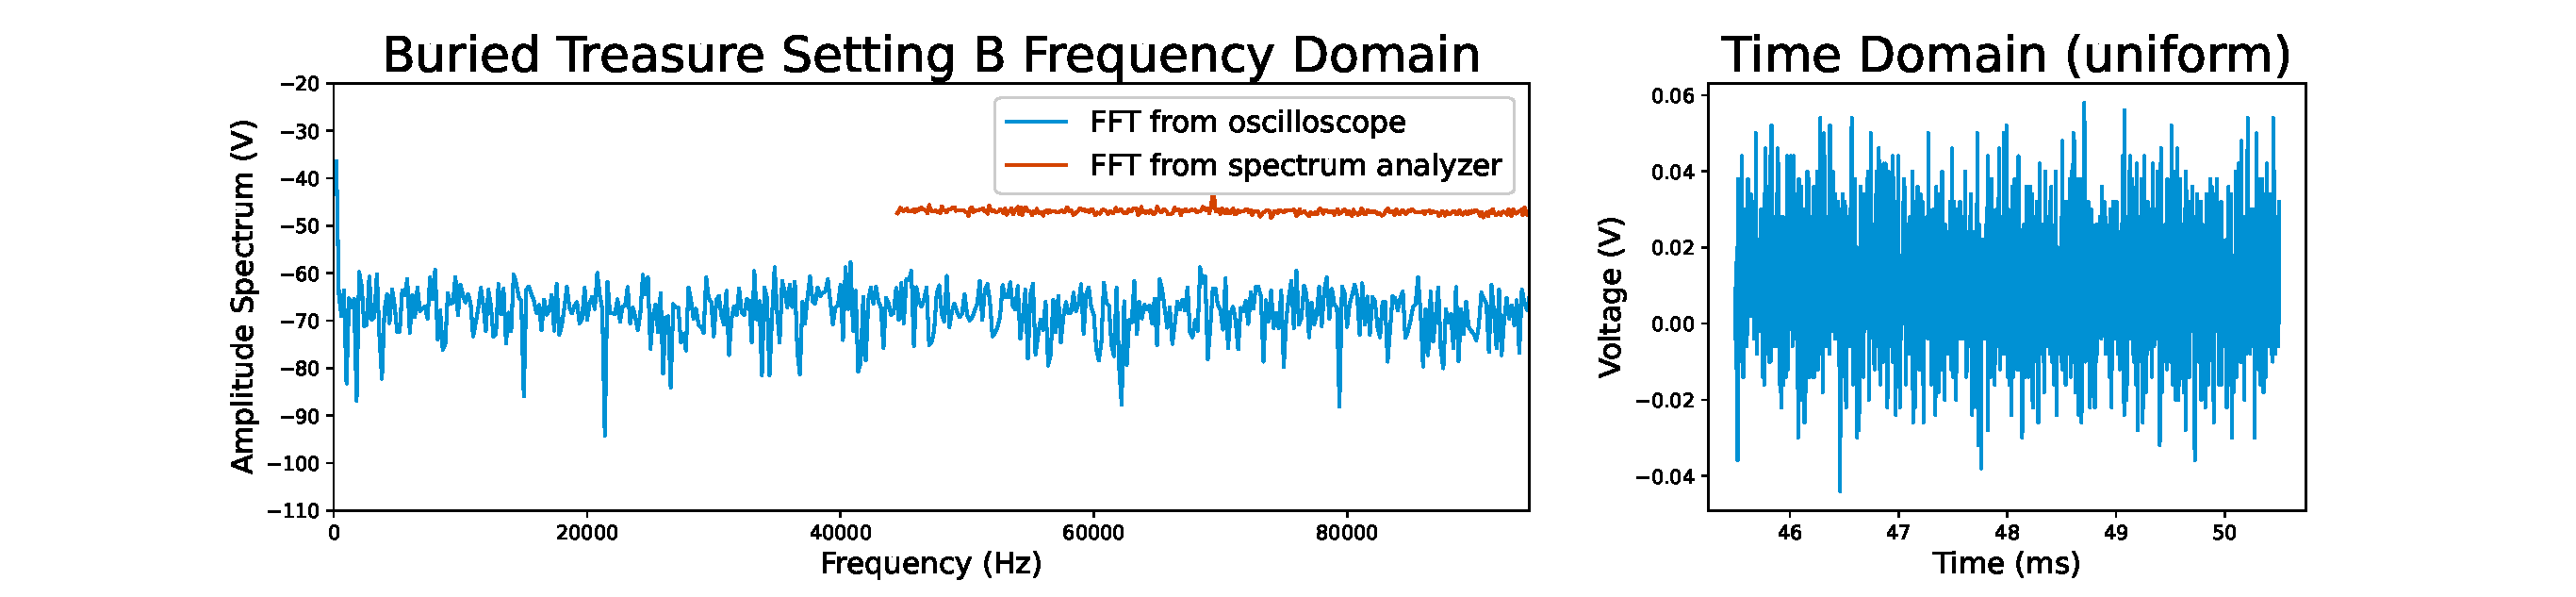
\includegraphics[width=\textwidth]{Buried Treasure Setting B (uniform)}
        \caption{}
        \label{fig:buried B}
        \end{subfigure}
        \begin{subfigure}[h]{\textwidth}
        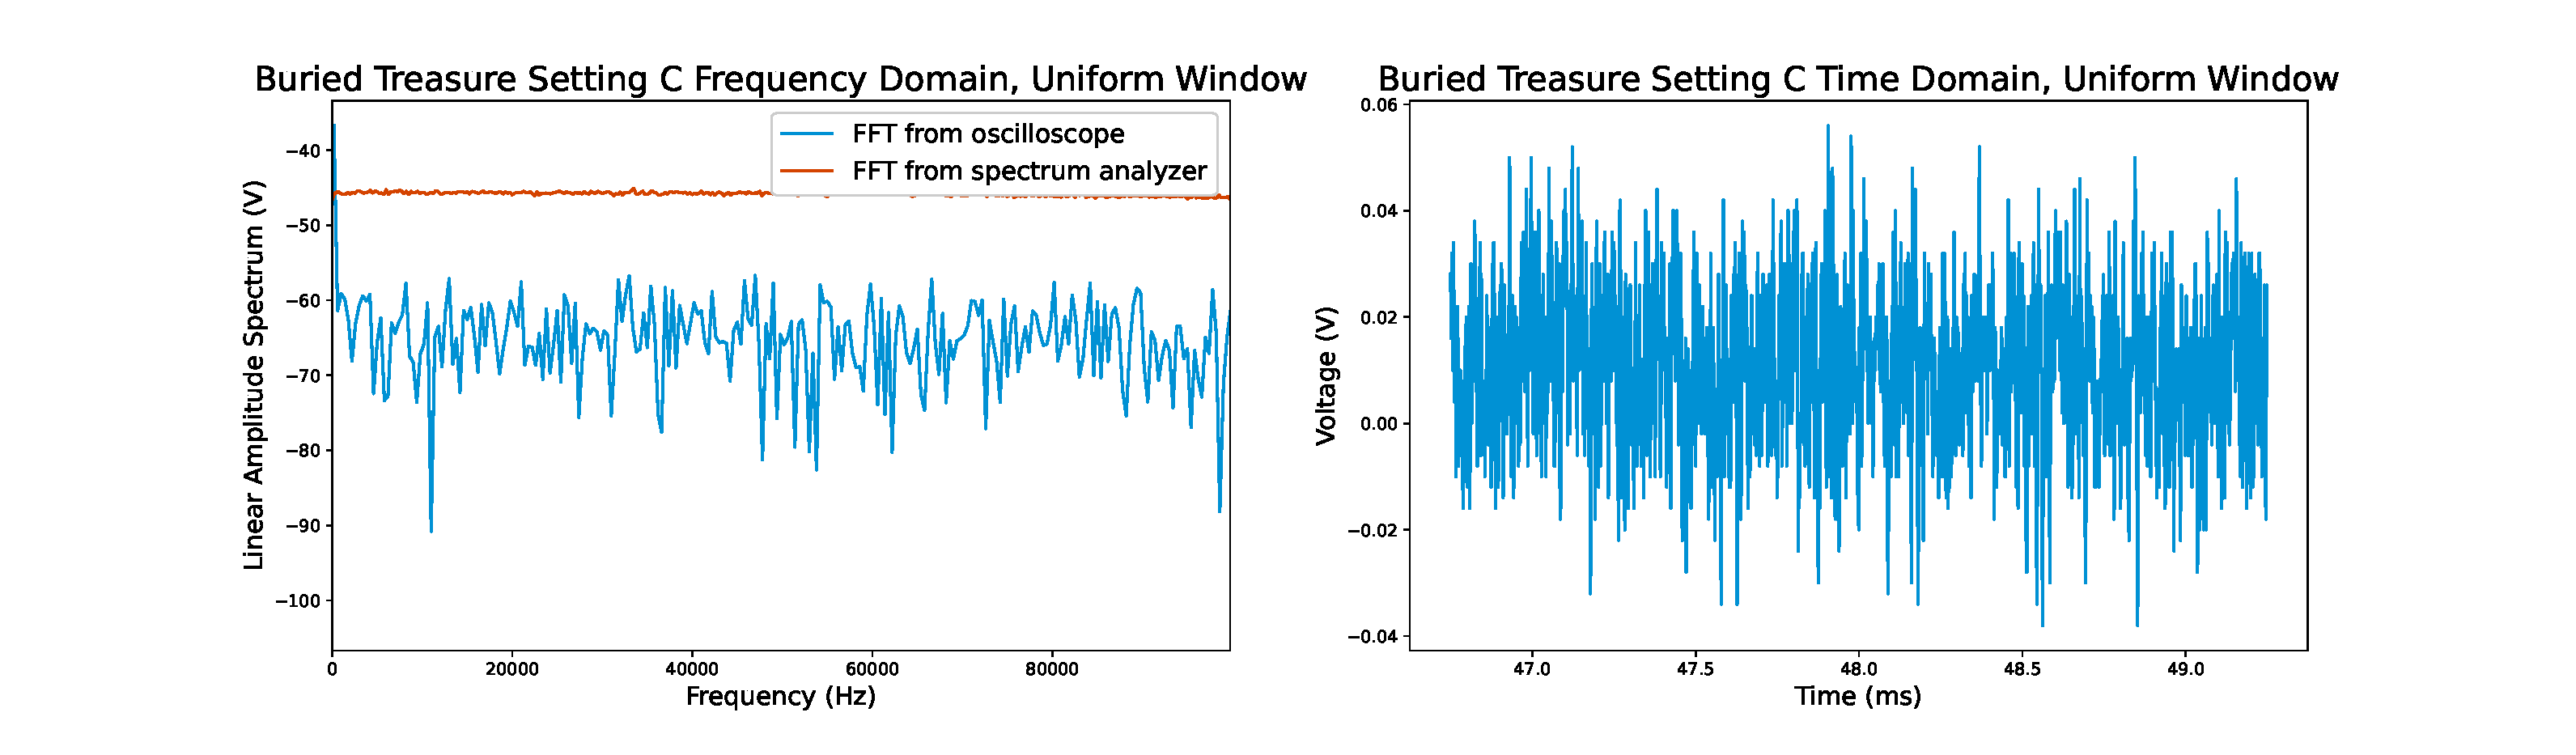
\includegraphics[width=\textwidth]{Buried Treasure Setting C (uniform)}
        \caption{}
        \label{fig:buried C}
        \end{subfigure}
    \end{figure} % buried treasure
    \subsection{LRC Analysis}
    
    \begin{figure}
    \centering
        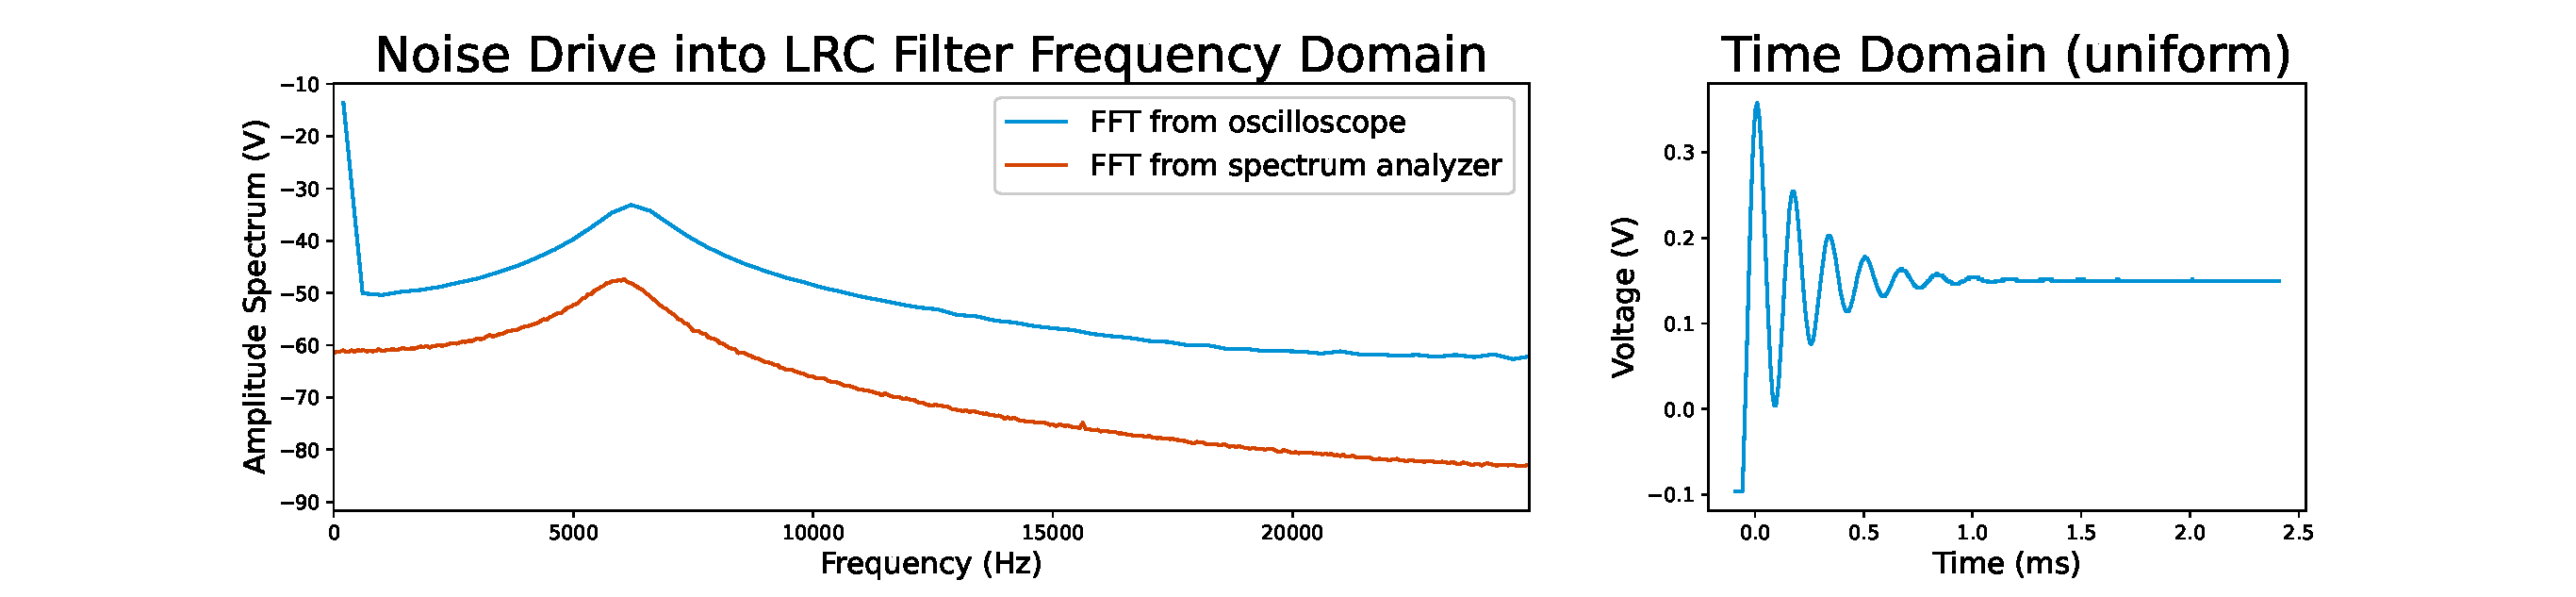
\includegraphics[width=\textwidth]{Noise Drive into LRC Filter (uniform)}
        \caption{}
        \label{fig:LRC fft}
    \end{figure} % LRC FFT
    
    \begin{figure}
    \centering
        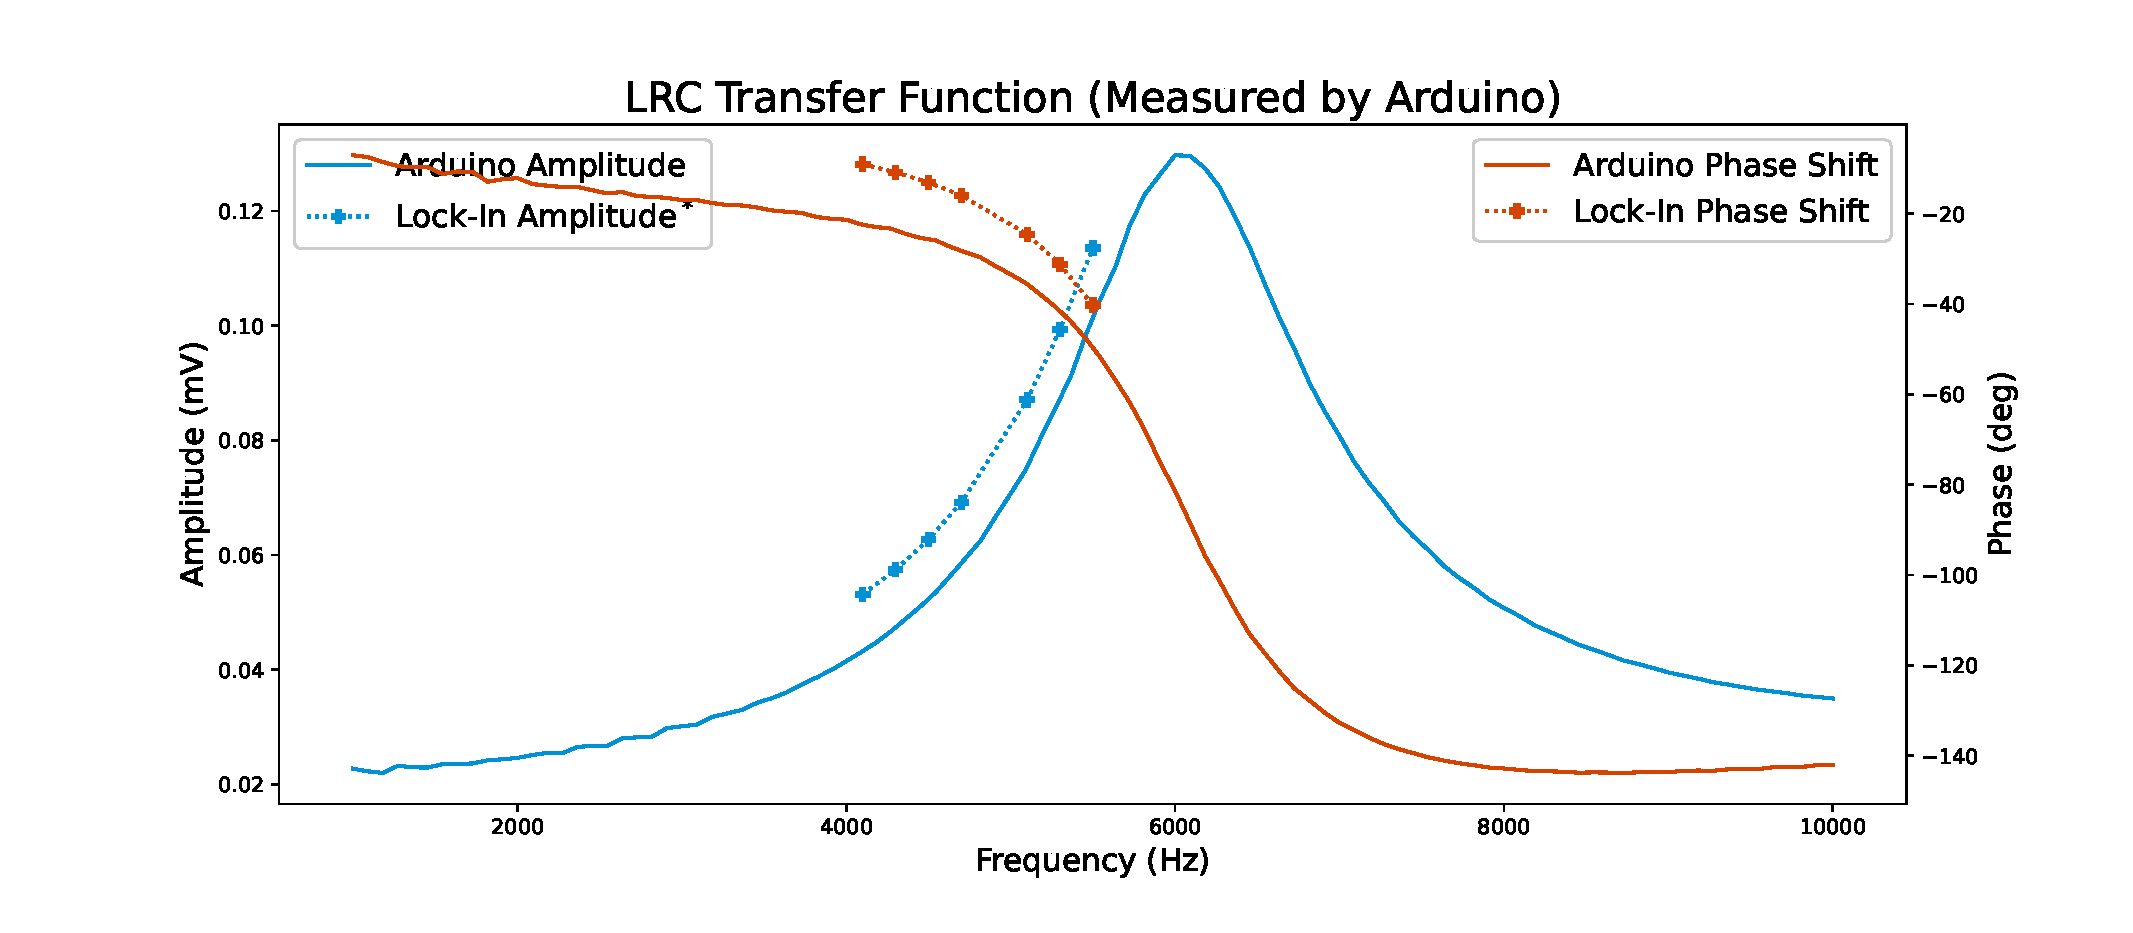
\includegraphics[width=\textwidth]{arduino data_}
        \caption{}
        \label{fig:LRC Arduino}
    \end{figure} % LRC Arduino
    
    \subsection{Acoustical Cavity Analysis}
    
    % \begin{figure}
    % \begin{subfigure}
    %     \centering
    %     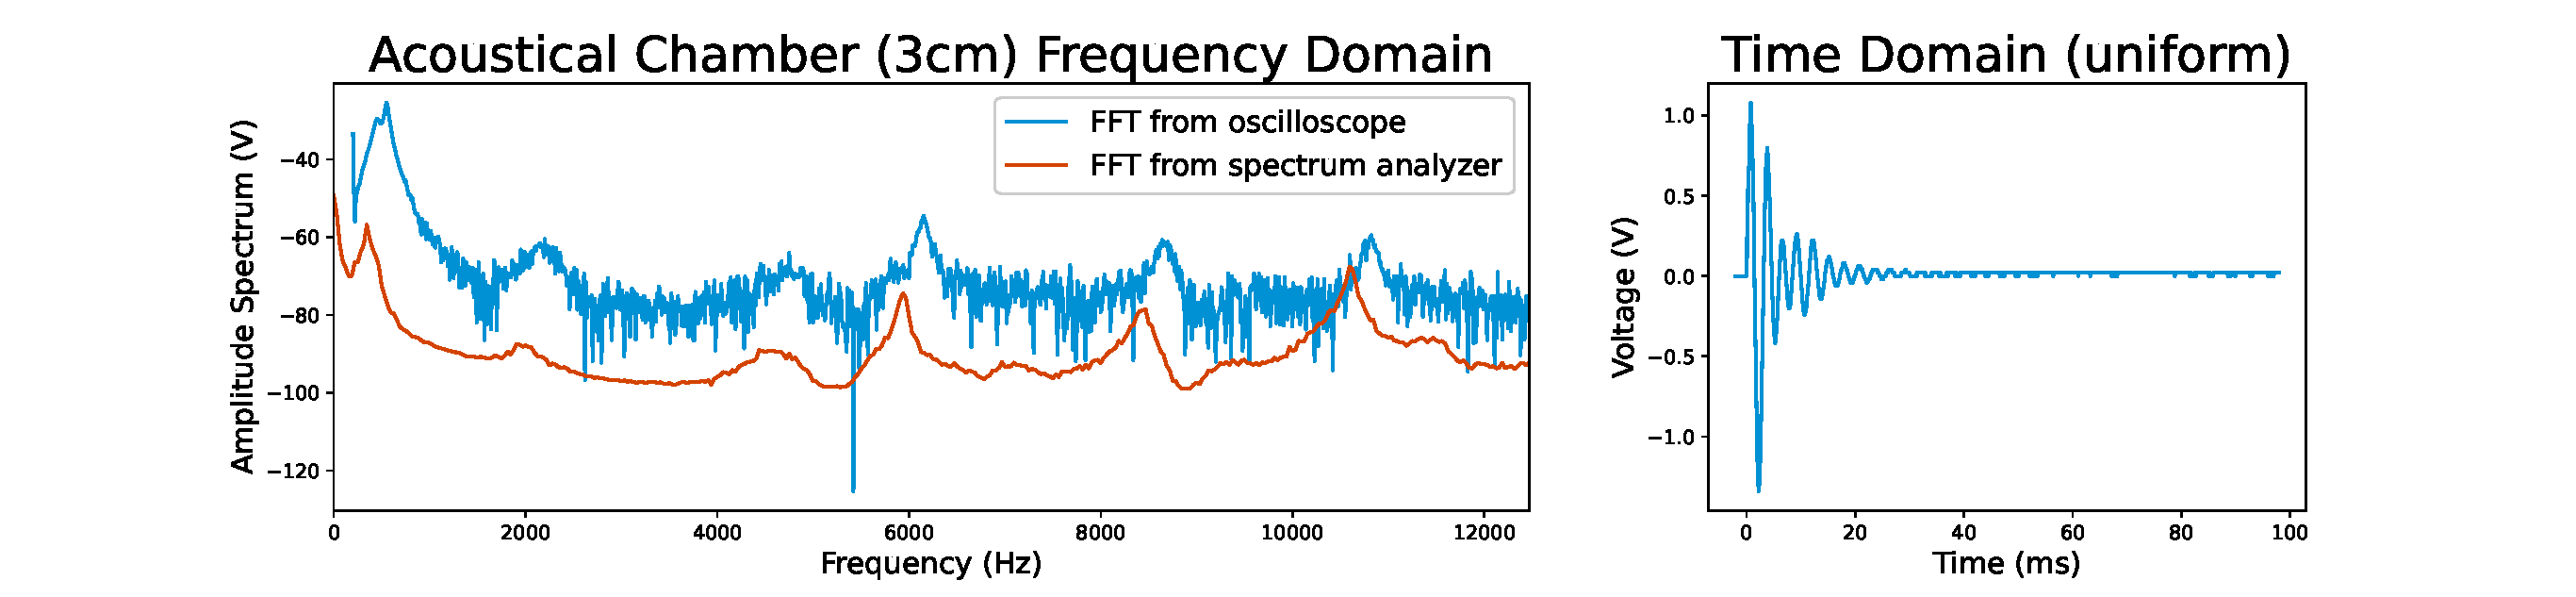
\includegraphics[width=\textwidth]{Acoustical Chamber (3cm) (uniform)}
    %     \caption{}
    %     \label{fig:AC fft 3}
    % \end{subfigure}
    % \begin{subfigure}
    %     \centering
    %     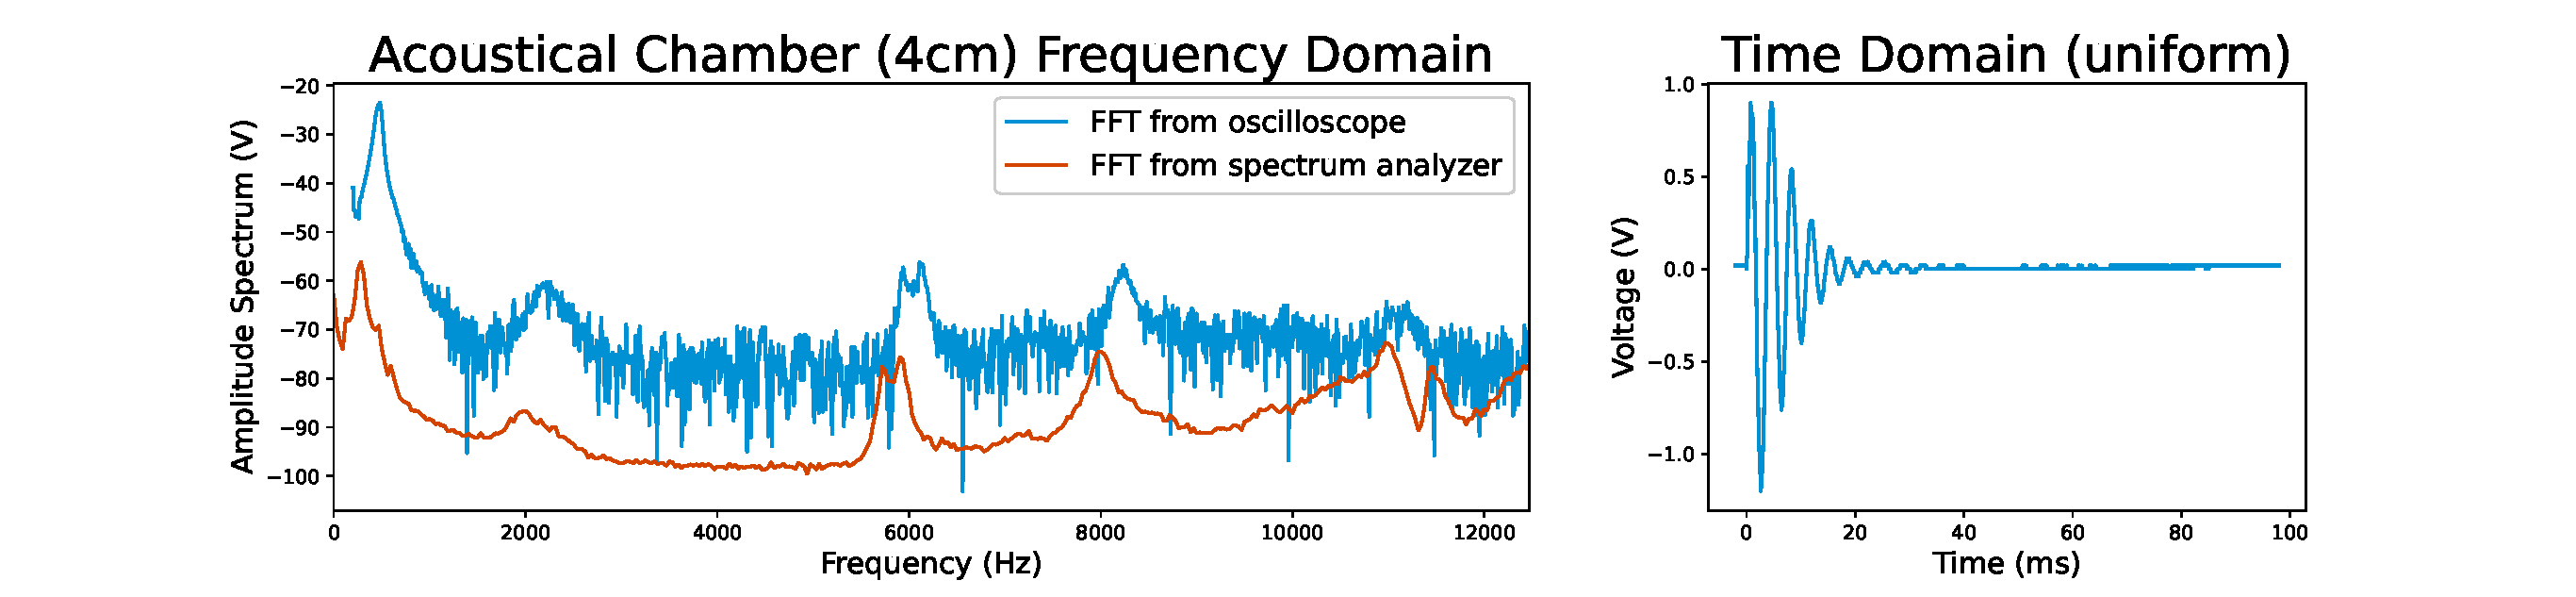
\includegraphics[width=\textwidth]{Acoustical Chamber (4cm) (uniform)}
    %     \caption{}
    %     \label{fig:AC fft 4}
    % \end{subfigure}
    % \begin{subfigure}
    %     \centering
    %     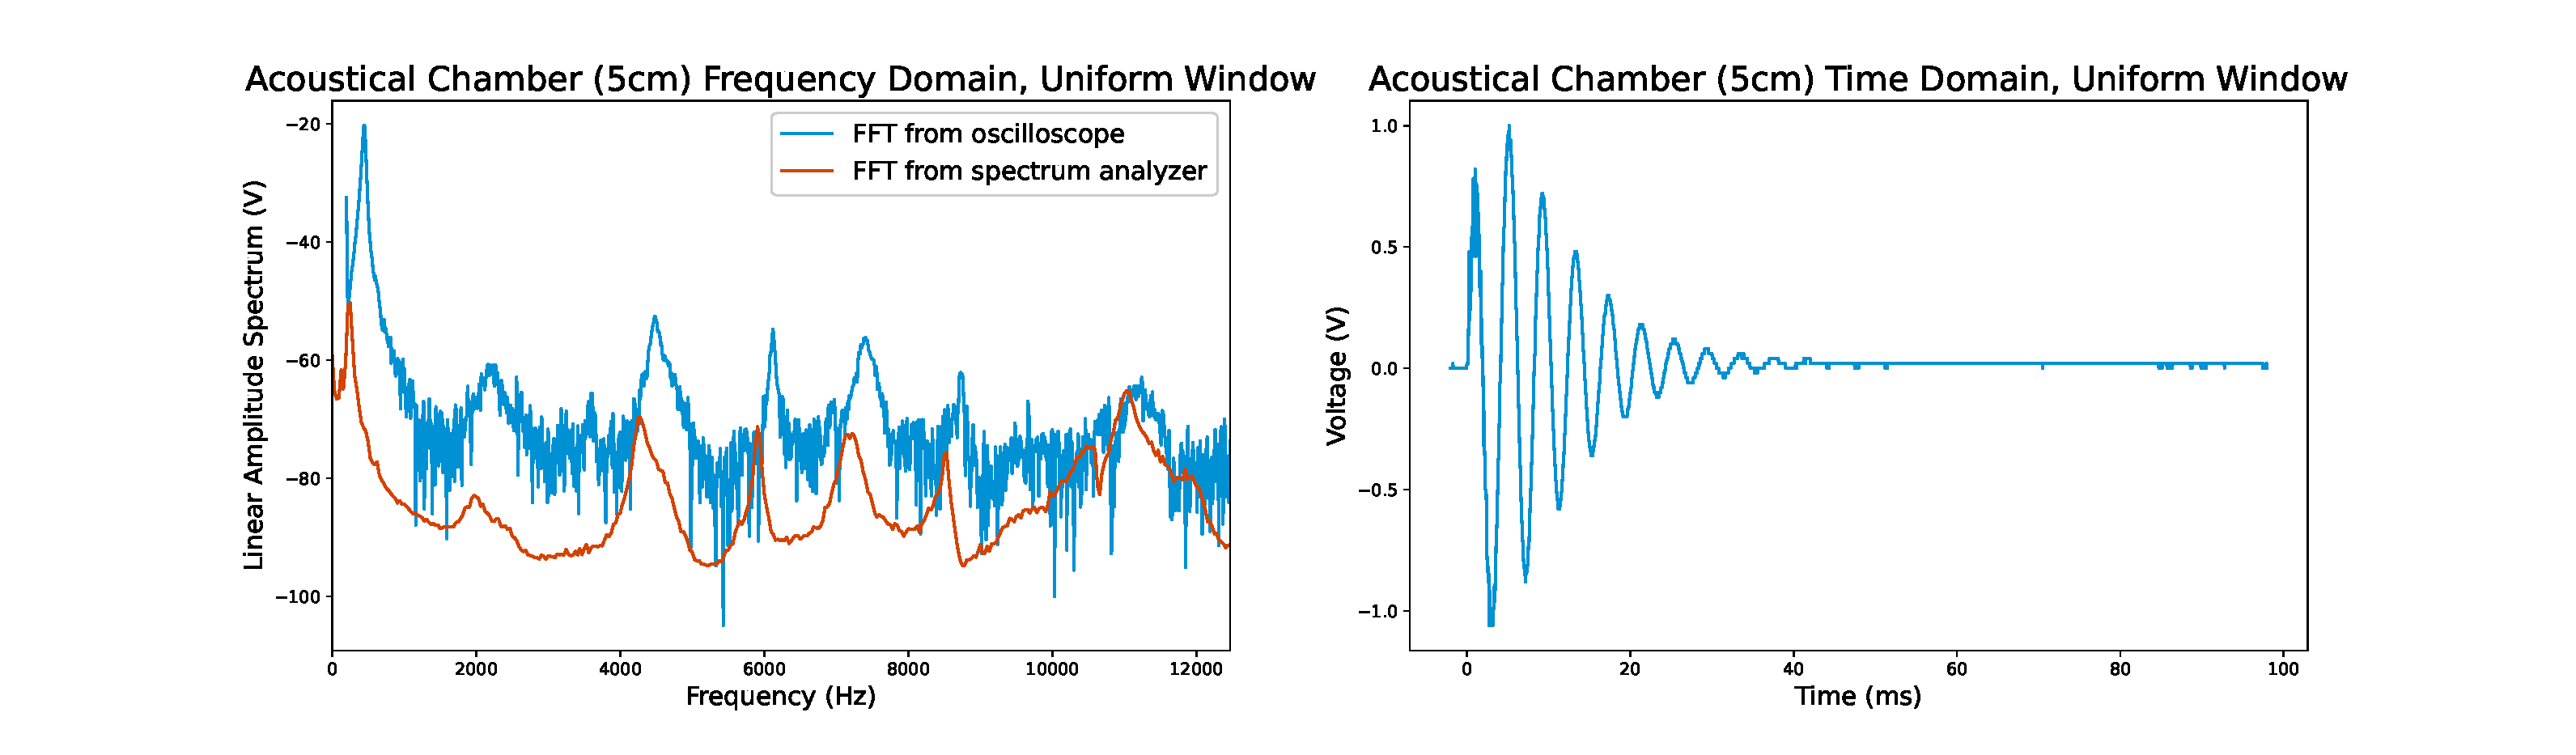
\includegraphics[width=\textwidth]{Acoustical Chamber (5cm) (uniform)}
    %     \caption{}
    %     \label{fig:AC fft 5}
    % \end{subfigure}
    % \begin{subfigure}
    %     \centering
    %     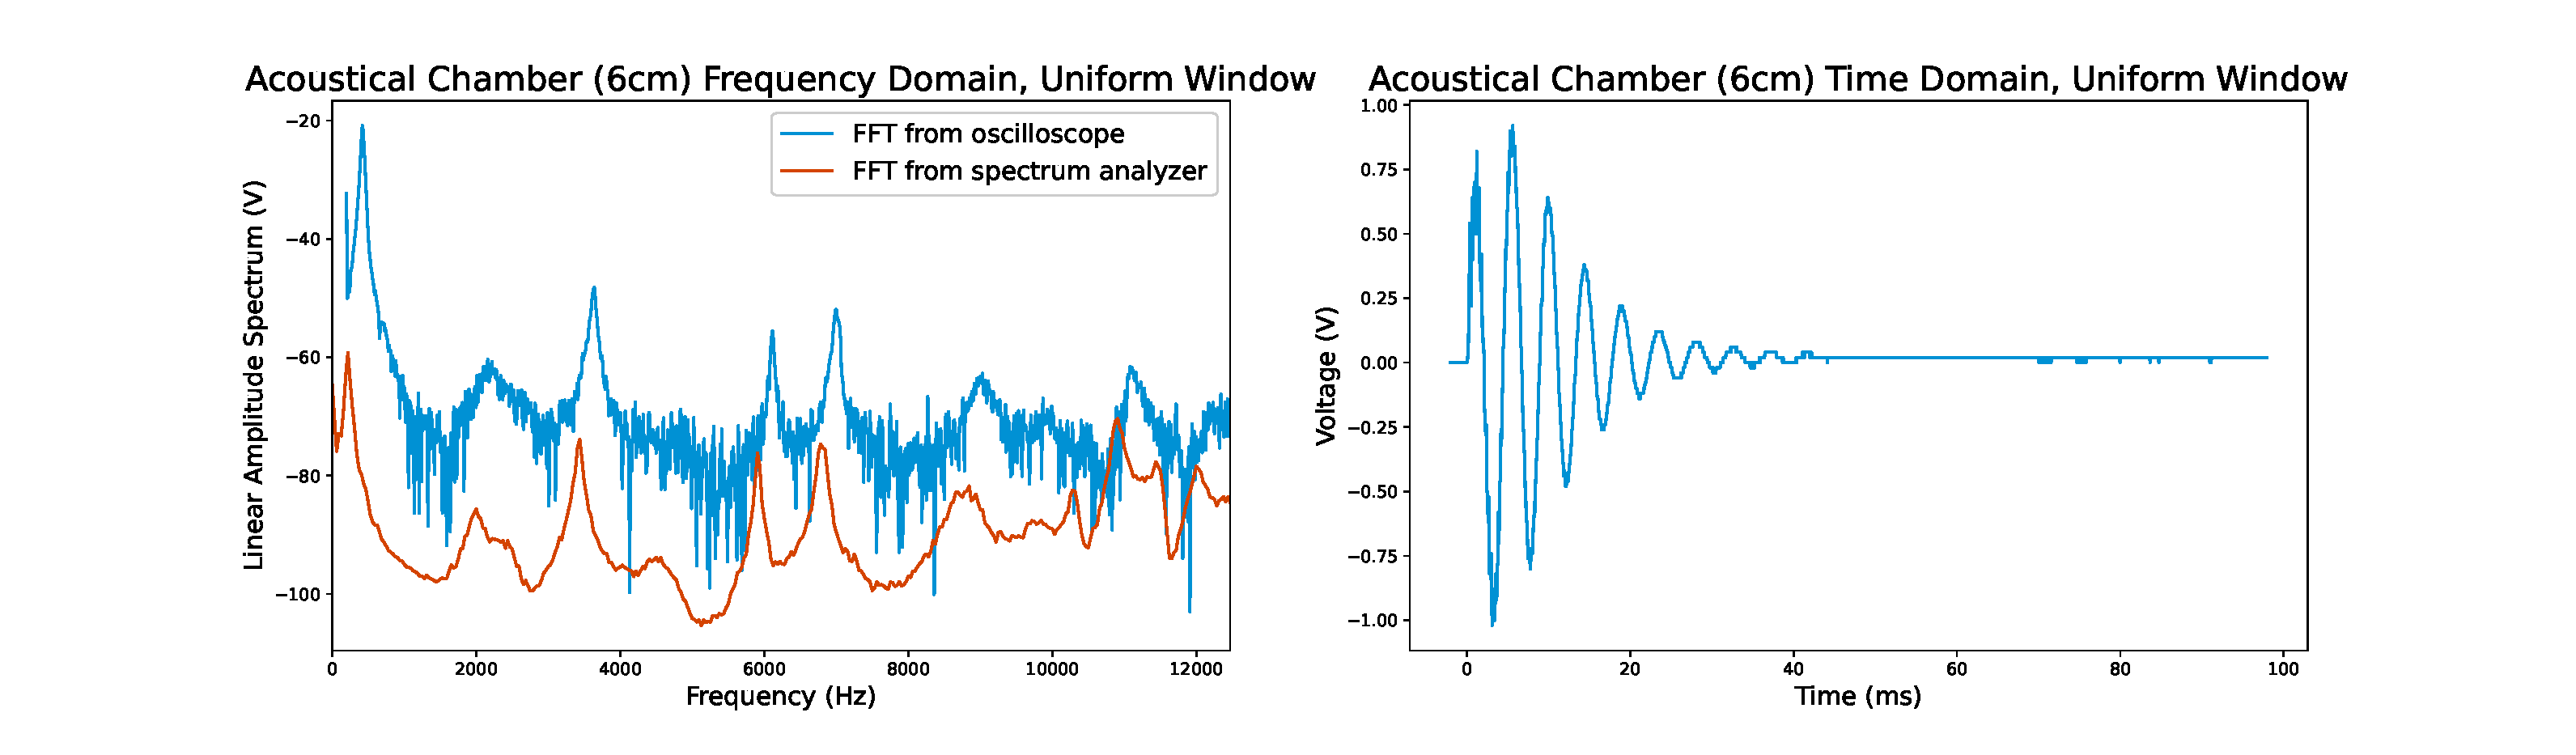
\includegraphics[width=\textwidth]{Acoustical Chamber (6cm) (uniform)}
    %     \caption{}
    %     \label{fig:AC fft 6}
    % \end{subfigure}
    % \end{figure} % AC FFT
    
    % \begin{figure}
    % \begin{subfigure}
    %     \centering
    %     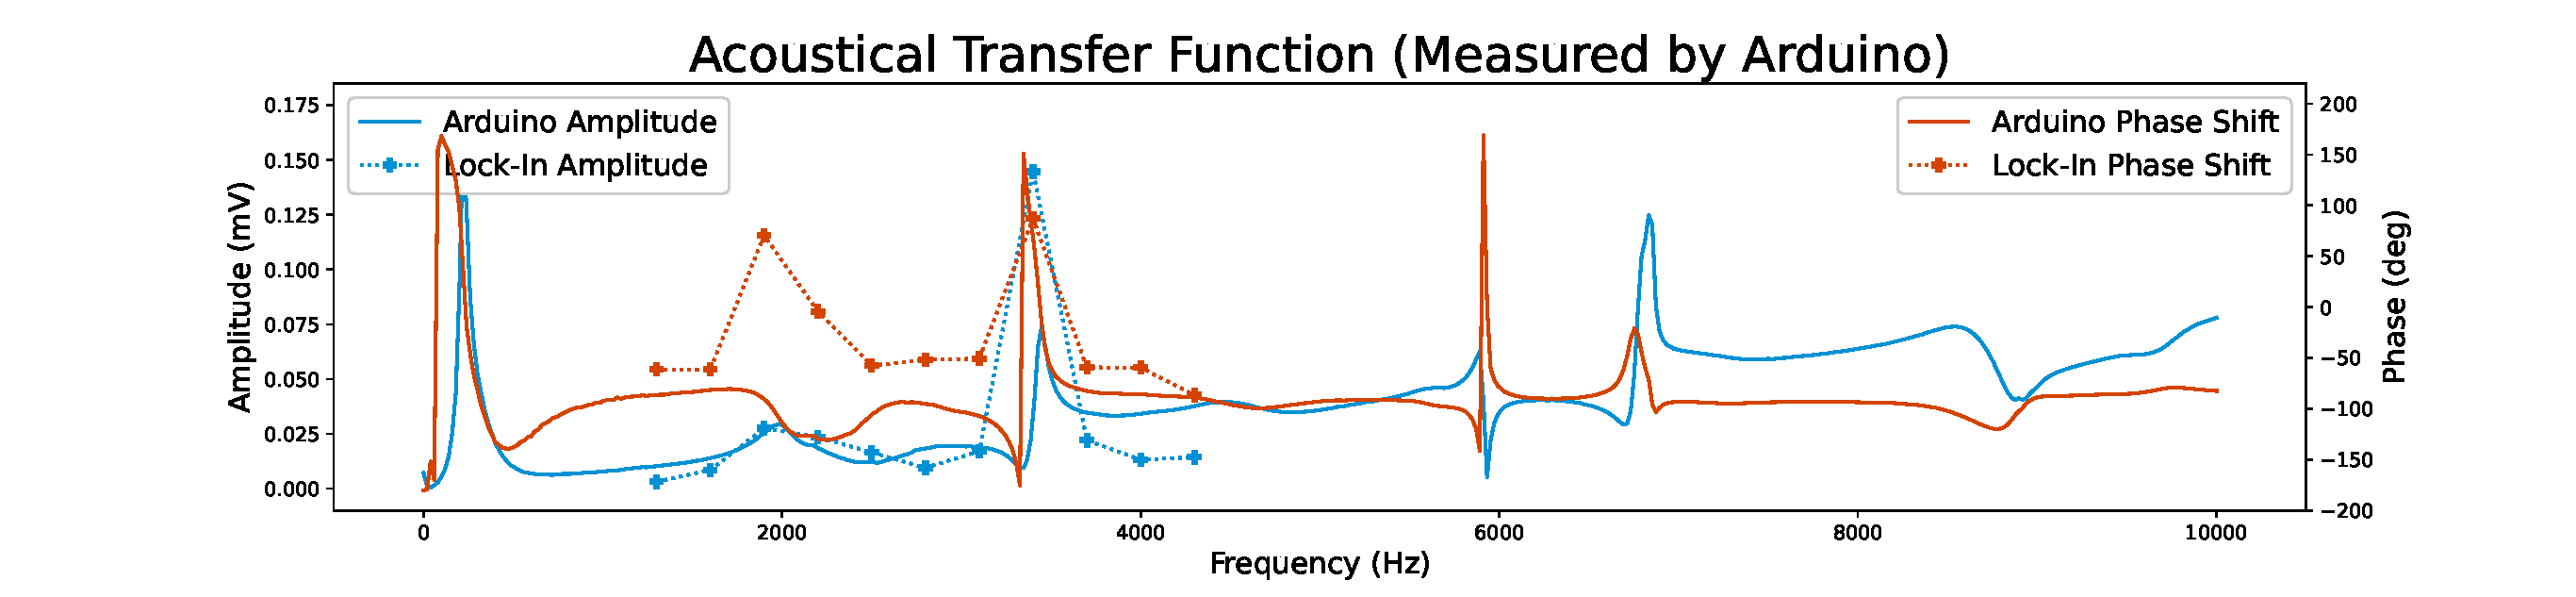
\includegraphics[width=\textwidth]{arduino data_0}
    %     \caption{}
    %     \label{fig:AC Arduino 0}
    % \end{subfigure}
    % \begin{subfigure}
    %     \centering
    %     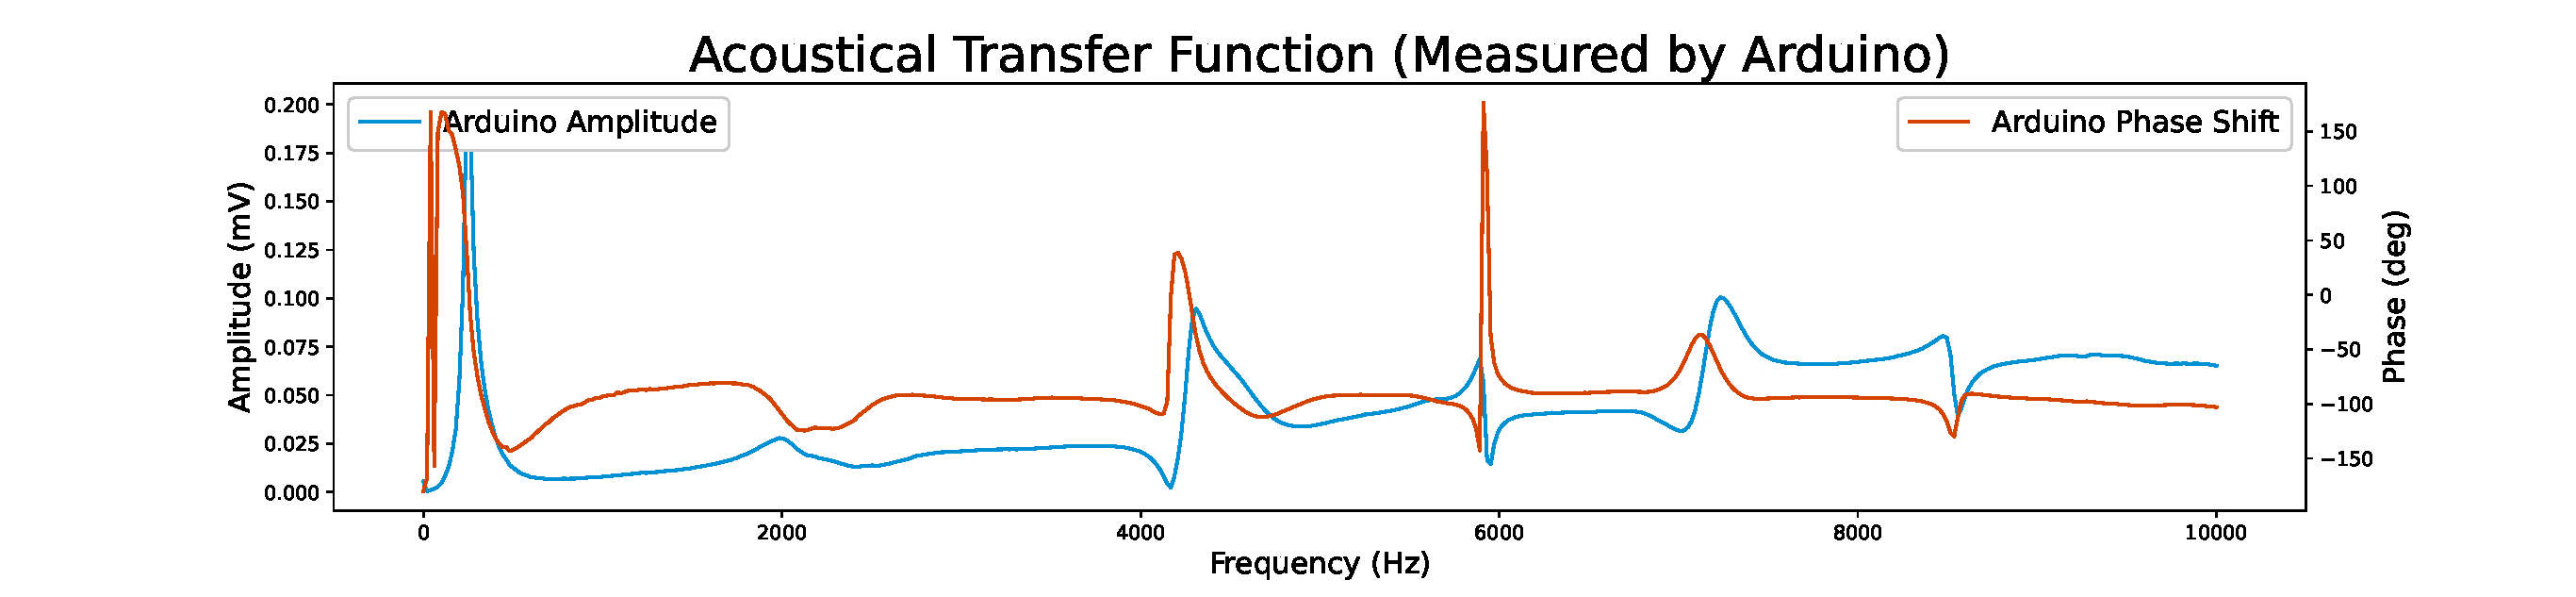
\includegraphics[width=\textwidth]{arduino data_1}
    %     \caption{}
    %     \label{fig:AC Arduino 1}
    % \end{subfigure}
    % \begin{subfigure}
    %     \centering
    %     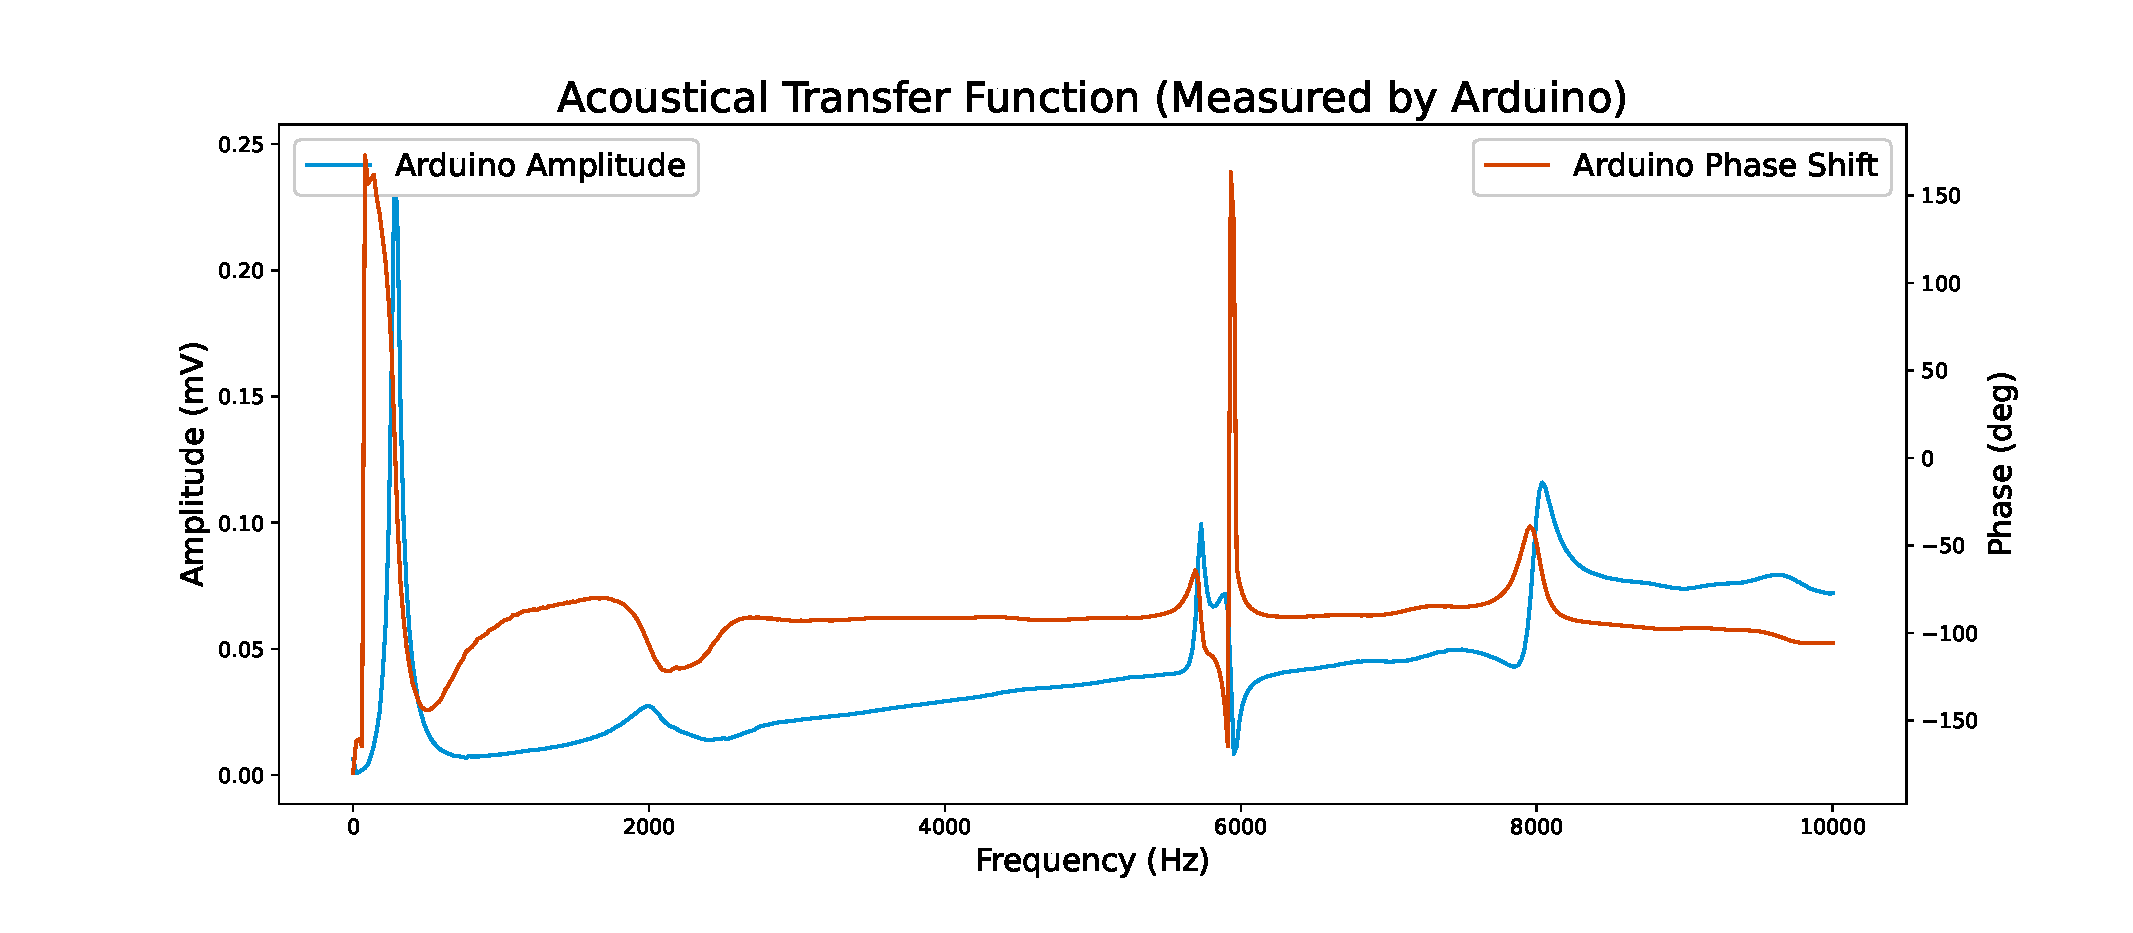
\includegraphics[width=\textwidth]{arduino data_2}
    %     \caption{}
    %     \label{fig:AC Arduino 2}
    % \end{subfigure}
    % \end{figure} % AC Arduino
    
    \section{Discussion and Conclusions}
    
    % \bibliographystyle{unsrt}
    % \bibliography{references}
    
    % \begin{thebibliography}{1}
    
    % \bibitem{manual} Foundational Magnetic Susceptibility Manual. Teach Spin. Manual provided in lab.
    
    % \bibitem{grav} “Gravity at Bozeman, Mt.” Www.wolframalpha.com, Wolfram Alpha LLC, www.wolframalpha.com/input/?i=gravity+at+bozeman$\%$2C+mt. Accessed 3 Oct. 2021.
    
    % \bibitem{molar} Molar Mass Calculator, https://www.webqc.org/, 10/03/2021
    
    % \bibitem{molar2} Molecular weight and molar mass for chemistry problems,
    % https://www.convertunits.com/molarmass/, 10/03/2021
    
    % \bibitem{himalayan salt} Themeadow.com. 2021. Minerals in Himalayan Pink Salt: Spectral Analysis | The Meadow. [online] Available at: <https://themeadow.com/pages/minerals-in-himalayan-pink-salt-spectral-analysis> [Accessed 3 October 2021].
    
    % \bibitem{teachspin}“Foundational Magnetic Susceptibility.” TeachSpin, www.teachspin.com/fms.
    
    
    % \end{thebibliography}
    \newpage
    \section*{Appendix A}
        
    \begin{table}[h]
    \centering
        \begin{tabular}{llll}
        Freq & X      & Y      & Amp \\
        4.1  & 183.69 & 29.24  & 560 \\
        4.3  & 197.54 & 37.87  & 600 \\
        4.5  & 213.8  & 49.68  & 650 \\
        4.7  & 232.8  & 66.59  & 720 \\
        4.9  & 254.3  & 90.76  & 790 \\
        5.1  & 277.2  & 126.8  & 880 \\
        5.3  & 297.2  & 180.24 & 1010\\
        5.5  & 303.3  & 257.2  & 1140\\
        5.5  & 303.7  & 256.4  & 1140\\
        \end{tabular}
        \caption{sin lock-in/osci LRC}
        \label{tab:lock_in_LRC}
    \end{table}
    
    
    \end{document}
